
%% bare_jrnl.tex
%% V1.3
%% 2007/01/11
%% by Michael Shell
%% see http://www.michaelshell.org/
%% for current contact information.
%%
%% This is a skeleton file demonstrating the use of IEEEtran.cls
%% (requires IEEEtran.cls version 1.7 or later) with an IEEE journal paper.
%%
%% Support sites:
%% http://www.michaelshell.org/tex/ieeetran/
%% http://www.ctan.org/tex-archive/macros/latex/contrib/IEEEtran/
%% and
%% http://www.ieee.org/



% *** Authors should verify (and, if needed, correct) their LaTeX system  ***
% *** with the testflow diagnostic prior to trusting their LaTeX platform ***
% *** with production work. IEEE's font choices can trigger bugs that do  ***
% *** not appear when using other class files.                            ***
% The testflow support page is at:
% http://www.michaelshell.org/tex/testflow/


%%*************************************************************************
%% Legal Notice:
%% This code is offered as-is without any warranty either expressed or
%% implied; without even the implied warranty of MERCHANTABILITY or
%% FITNESS FOR A PARTICULAR PURPOSE!
%% User assumes all risk.
%% In no event shall IEEE or any contributor to this code be liable for
%% any damages or losses, including, but not limited to, incidental,
%% consequential, or any other damages, resulting from the use or misuse
%% of any information contained here.
%%
%% All comments are the opinions of their respective authors and are not
%% necessarily endorsed by the IEEE.
%%
%% This work is distributed under the LaTeX Project Public License (LPPL)
%% ( http://www.latex-project.org/ ) version 1.3, and may be freely used,
%% distributed and modified. A copy of the LPPL, version 1.3, is included
%% in the base LaTeX documentation of all distributions of LaTeX released
%% 2003/12/01 or later.
%% Retain all contribution notices and credits.
%% ** Modified files should be clearly indicated as such, including  **
%% ** renaming them and changing author support contact information. **
%%
%% File list of work: IEEEtran.cls, IEEEtran_HOWTO.pdf, bare_adv.tex,
%%                    bare_conf.tex, bare_jrnl.tex, bare_jrnl_compsoc.tex
%%*************************************************************************

% Note that the a4paper option is mainly intended so that authors in
% countries using A4 can easily print to A4 and see how their papers will
% look in print - the typesetting of the document will not typically be
% affected with changes in paper size (but the bottom and side margins will).
% Use the testflow package mentioned above to verify correct handling of
% both paper sizes by the user's LaTeX system.
%
% Also note that the "draftcls" or "draftclsnofoot", not "draft", option
% should be used if it is desired that the figures are to be displayed in
% draft mode.
%
\documentclass[journal]{IEEEtran}
%
% If IEEEtran.cls has not been installed into the LaTeX system files,
% manually specify the path to it like:
% \documentclass[journal]{../sty/IEEEtran}





% Some very useful LaTeX packages include:
% (uncomment the ones you want to load)


% *** MISC UTILITY PACKAGES ***
%
%\usepackage{ifpdf}
% Heiko Oberdiek's ifpdf.sty is very useful if you need conditional
% compilation based on whether the output is pdf or dvi.
% usage:
% \ifpdf
%   % pdf code
% \else
%   % dvi code
% \fi
% The latest version of ifpdf.sty can be obtained from:
% http://www.ctan.org/tex-archive/macros/latex/contrib/oberdiek/
% Also, note that IEEEtran.cls V1.7 and later provides a builtin
% \ifCLASSINFOpdf conditional that works the same way.
% When switching from latex to pdflatex and vice-versa, the compiler may
% have to be run twice to clear warning/error messages.






% *** CITATION PACKAGES ***
%
\usepackage{cite}
% cite.sty was written by Donald Arseneau
% V1.6 and later of IEEEtran pre-defines the format of the cite.sty package
% \cite{} output to follow that of IEEE. Loading the cite package will
% result in citation numbers being automatically sorted and properly
% "compressed/ranged". e.g., [1], [9], [2], [7], [5], [6] without using
% cite.sty will become [1], [2], [5]--[7], [9] using cite.sty. cite.sty's
% \cite will automatically add leading space, if needed. Use cite.sty's
% noadjust option (cite.sty V3.8 and later) if you want to turn this off.
% cite.sty is already installed on most LaTeX systems. Be sure and use
% version 4.0 (2003-05-27) and later if using hyperref.sty. cite.sty does
% not currently provide for hyperlinked citations.
% The latest version can be obtained at:
% http://www.ctan.org/tex-archive/macros/latex/contrib/cite/
% The documentation is contained in the cite.sty file itself.






% *** GRAPHICS RELATED PACKAGES ***
%
\ifCLASSINFOpdf
   \usepackage[pdftex]{graphicx}
  % declare the path(s) where your graphic files are
  % \graphicspath{{../pdf/}{../jpeg/}}
  % and their extensions so you won't have to specify these with
  % every instance of \includegraphics
  % \DeclareGraphicsExtensions{.pdf,.jpeg,.png}
\else
  % or other class option (dvipsone, dvipdf, if not using dvips). graphicx
  % will default to the driver specified in the system graphics.cfg if no
  % driver is specified.
   \usepackage[dvips]{graphicx}
  % declare the path(s) where your graphic files are
  % \graphicspath{{../eps/}}
  % and their extensions so you won't have to specify these with
  % every instance of \includegraphics
  % \DeclareGraphicsExtensions{.eps}
\fi
% graphicx was written by David Carlisle and Sebastian Rahtz. It is
% required if you want graphics, photos, etc. graphicx.sty is already
% installed on most LaTeX systems. The latest version and documentation can
% be obtained at:
% http://www.ctan.org/tex-archive/macros/latex/required/graphics/
% Another good source of documentation is "Using Imported Graphics in
% LaTeX2e" by Keith Reckdahl which can be found as epslatex.ps or
% epslatex.pdf at: http://www.ctan.org/tex-archive/info/
%
% latex, and pdflatex in dvi mode, support graphics in encapsulated
% postscript (.eps) format. pdflatex in pdf mode supports graphics
% in .pdf, .jpeg, .png and .mps (metapost) formats. Users should ensure
% that all non-photo figures use a vector format (.eps, .pdf, .mps) and
% not a bitmapped formats (.jpeg, .png). IEEE frowns on bitmapped formats
% which can result in "jaggedy"/blurry rendering of lines and letters as
% well as large increases in file sizes.
%
% You can find documentation about the pdfTeX application at:
% http://www.tug.org/applications/pdftex





% *** MATH PACKAGES ***
%
\usepackage[cmex10]{amsmath}
\usepackage{amssymb}
% A popular package from the American Mathematical Society that provides
% many useful and powerful commands for dealing with mathematics. If using
% it, be sure to load this package with the cmex10 option to ensure that
% only type 1 fonts will utilized at all point sizes. Without this option,
% it is possible that some math symbols, particularly those within
% footnotes, will be rendered in bitmap form which will result in a
% document that can not be IEEE Xplore compliant!
%
% Also, note that the amsmath package sets \interdisplaylinepenalty to 10000
% thus preventing page breaks from occurring within multiline equations. Use:
%\interdisplaylinepenalty=2500
% after loading amsmath to restore such page breaks as IEEEtran.cls normally
% does. amsmath.sty is already installed on most LaTeX systems. The latest
% version and documentation can be obtained at:
% http://www.ctan.org/tex-archive/macros/latex/required/amslatex/math/




\usepackage{algorithm}
\usepackage{algorithmic}

% *** SPECIALIZED LIST PACKAGES ***
%
%\usepackage{algorithmic}
% algorithmic.sty was written by Peter Williams and Rogerio Brito.
% This package provides an algorithmic environment fo describing algorithms.
% You can use the algorithmic environment in-text or within a figure
% environment to provide for a floating algorithm. Do NOT use the algorithm
% floating environment provided by algorithm.sty (by the same authors) or
% algorithm2e.sty (by Christophe Fiorio) as IEEE does not use dedicated
% algorithm float types and packages that provide these will not provide
% correct IEEE style captions. The latest version and documentation of
% algorithmic.sty can be obtained at:
% http://www.ctan.org/tex-archive/macros/latex/contrib/algorithms/
% There is also a support site at:
% http://algorithms.berlios.de/index.html
% Also of interest may be the (relatively newer and more customizable)
% algorithmicx.sty package by Szasz Janos:
% http://www.ctan.org/tex-archive/macros/latex/contrib/algorithmicx/




% *** ALIGNMENT PACKAGES ***
%
%\usepackage{array}
% Frank Mittelbach's and David Carlisle's array.sty patches and improves
% the standard LaTeX2e array and tabular environments to provide better
% appearance and additional user controls. As the default LaTeX2e table
% generation code is lacking to the point of almost being broken with
% respect to the quality of the end results, all users are strongly
% advised to use an enhanced (at the very least that provided by array.sty)
% set of table tools. array.sty is already installed on most systems. The
% latest version and documentation can be obtained at:
% http://www.ctan.org/tex-archive/macros/latex/required/tools/


%\usepackage{mdwmath}
%\usepackage{mdwtab}
% Also highly recommended is Mark Wooding's extremely powerful MDW tools,
% especially mdwmath.sty and mdwtab.sty which are used to format equations
% and tables, respectively. The MDWtools set is already installed on most
% LaTeX systems. The lastest version and documentation is available at:
% http://www.ctan.org/tex-archive/macros/latex/contrib/mdwtools/


% IEEEtran contains the IEEEeqnarray family of commands that can be used to
% generate multiline equations as well as matrices, tables, etc., of high
% quality.


%\usepackage{eqparbox}
% Also of notable interest is Scott Pakin's eqparbox package for creating
% (automatically sized) equal width boxes - aka "natural width parboxes".
% Available at:
% http://www.ctan.org/tex-archive/macros/latex/contrib/eqparbox/





% *** SUBFIGURE PACKAGES ***
%\usepackage[tight,footnotesize]{subfigure}
% subfigure.sty was written by Steven Douglas Cochran. This package makes it
% easy to put subfigures in your figures. e.g., "Figure 1a and 1b". For IEEE
% work, it is a good idea to load it with the tight package option to reduce
% the amount of white space around the subfigures. subfigure.sty is already
% installed on most LaTeX systems. The latest version and documentation can
% be obtained at:
% http://www.ctan.org/tex-archive/obsolete/macros/latex/contrib/subfigure/
% subfigure.sty has been superceeded by subfig.sty.



%\usepackage[caption=false]{caption}
%\usepackage[font=footnotesize]{subfig}
% subfig.sty, also written by Steven Douglas Cochran, is the modern
% replacement for subfigure.sty. However, subfig.sty requires and
% automatically loads Axel Sommerfeldt's caption.sty which will override
% IEEEtran.cls handling of captions and this will result in nonIEEE style
% figure/table captions. To prevent this problem, be sure and preload
% caption.sty with its "caption=false" package option. This is will preserve
% IEEEtran.cls handing of captions. Version 1.3 (2005/06/28) and later
% (recommended due to many improvements over 1.2) of subfig.sty supports
% the caption=false option directly:
%\usepackage[caption=false,font=footnotesize]{subfig}
%
% The latest version and documentation can be obtained at:
% http://www.ctan.org/tex-archive/macros/latex/contrib/subfig/
% The latest version and documentation of caption.sty can be obtained at:
% http://www.ctan.org/tex-archive/macros/latex/contrib/caption/




% *** FLOAT PACKAGES ***
%
%\usepackage{fixltx2e}
% fixltx2e, the successor to the earlier fix2col.sty, was written by
% Frank Mittelbach and David Carlisle. This package corrects a few problems
% in the LaTeX2e kernel, the most notable of which is that in current
% LaTeX2e releases, the ordering of single and double column floats is not
% guaranteed to be preserved. Thus, an unpatched LaTeX2e can allow a
% single column figure to be placed prior to an earlier double column
% figure. The latest version and documentation can be found at:
% http://www.ctan.org/tex-archive/macros/latex/base/



%\usepackage{stfloats}
% stfloats.sty was written by Sigitas Tolusis. This package gives LaTeX2e
% the ability to do double column floats at the bottom of the page as well
% as the top. (e.g., "\begin{figure*}[!b]" is not normally possible in
% LaTeX2e). It also provides a command:
%\fnbelowfloat
% to enable the placement of footnotes below bottom floats (the standard
% LaTeX2e kernel puts them above bottom floats). This is an invasive package
% which rewrites many portions of the LaTeX2e float routines. It may not work
% with other packages that modify the LaTeX2e float routines. The latest
% version and documentation can be obtained at:
% http://www.ctan.org/tex-archive/macros/latex/contrib/sttools/
% Documentation is contained in the stfloats.sty comments as well as in the
% presfull.pdf file. Do not use the stfloats baselinefloat ability as IEEE
% does not allow \baselineskip to stretch. Authors submitting work to the
% IEEE should note that IEEE rarely uses double column equations and
% that authors should try to avoid such use. Do not be tempted to use the
% cuted.sty or midfloat.sty packages (also by Sigitas Tolusis) as IEEE does
% not format its papers in such ways.


%\ifCLASSOPTIONcaptionsoff
%  \usepackage[nomarkers]{endfloat}
% \let\MYoriglatexcaption\caption
% \renewcommand{\caption}[2][\relax]{\MYoriglatexcaption[#2]{#2}}
%\fi
% endfloat.sty was written by James Darrell McCauley and Jeff Goldberg.
% This package may be useful when used in conjunction with IEEEtran.cls'
% captionsoff option. Some IEEE journals/societies require that submissions
% have lists of figures/tables at the end of the paper and that
% figures/tables without any captions are placed on a page by themselves at
% the end of the document. If needed, the draftcls IEEEtran class option or
% \CLASSINPUTbaselinestretch interface can be used to increase the line
% spacing as well. Be sure and use the nomarkers option of endfloat to
% prevent endfloat from "marking" where the figures would have been placed
% in the text. The two hack lines of code above are a slight modification of
% that suggested by in the endfloat docs (section 8.3.1) to ensure that
% the full captions always appear in the list of figures/tables - even if
% the user used the short optional argument of \caption[]{}.
% IEEE papers do not typically make use of \caption[]'s optional argument,
% so this should not be an issue. A similar trick can be used to disable
% captions of packages such as subfig.sty that lack options to turn off
% the subcaptions:
% For subfig.sty:
% \let\MYorigsubfloat\subfloat
% \renewcommand{\subfloat}[2][\relax]{\MYorigsubfloat[]{#2}}
% For subfigure.sty:
% \let\MYorigsubfigure\subfigure
% \renewcommand{\subfigure}[2][\relax]{\MYorigsubfigure[]{#2}}
% However, the above trick will not work if both optional arguments of
% the \subfloat/subfig command are used. Furthermore, there needs to be a
% description of each subfigure *somewhere* and endfloat does not add
% subfigure captions to its list of figures. Thus, the best approach is to
% avoid the use of subfigure captions (many IEEE journals avoid them anyway)
% and instead reference/explain all the subfigures within the main caption.
% The latest version of endfloat.sty and its documentation can obtained at:
% http://www.ctan.org/tex-archive/macros/latex/contrib/endfloat/
%
% The IEEEtran \ifCLASSOPTIONcaptionsoff conditional can also be used
% later in the document, say, to conditionally put the References on a
% page by themselves.





% *** PDF, URL AND HYPERLINK PACKAGES ***
%
\usepackage{url}
% url.sty was written by Donald Arseneau. It provides better support for
% handling and breaking URLs. url.sty is already installed on most LaTeX
% systems. The latest version can be obtained at:
% http://www.ctan.org/tex-archive/macros/latex/contrib/misc/
% Read the url.sty source comments for usage information. Basically,
% \url{my_url_here}.





% *** Do not adjust lengths that control margins, column widths, etc. ***
% *** Do not use packages that alter fonts (such as pslatex).         ***
% There should be no need to do such things with IEEEtran.cls V1.6 and later.
% (Unless specifically asked to do so by the journal or conference you plan
% to submit to, of course. )


% correct bad hyphenation here
\hyphenation{op-tical net-works semi-conduc-tor}

\makeatletter
\newcommand{\rmnum}[1]{\romannumeral #1}
\newcommand{\Rmnum}[1]{\expandafter\@slowromancap\romannumeral #1@}
\makeatother

\begin{document}
%
% paper title
% can use linebreaks \\ within to get better formatting as desired
\title{A Halting Algorithm to Determine the Existence of Decoder}
%
%
% author names and IEEE memberships
% note positions of commas and nonbreaking spaces ( ~ ) LaTeX will not break
% a structure at a ~ so this keeps an author's name from being broken across
% two lines.
% use \thanks{} to gain access to the first footnote area
% a separate \thanks must be used for each paragraph as LaTeX2e's \thanks
% was not built to handle multiple paragraphs
%

%\author{Michael~Shell,~\IEEEmembership{Member,~IEEE,}
%        John~Doe,~\IEEEmembership{Fellow,~OSA,}
%        and~Jane~Doe,~\IEEEmembership{Life~Fellow,~IEEE}% <-this % stops a space
%\thanks{M. Shell is with the Department
%of Electrical and Computer Engineering, Georgia Institute of Technology, Atlanta,
%GA, 30332 USA e-mail: (see http://www.michaelshell.org/contact.html).}% <-this % stops a space
%\thanks{J. Doe and J. Doe are with Anonymous University.}% <-this % stops a space
%\thanks{Manuscript received April 19, 2005; revised January 11, 2007.}}
\author{
\IEEEauthorblockN{ShengYu Shen, Ying Qin, JianMin Zhang, and SiKun Li}\\
\IEEEauthorblockA{School of Computer Science, National
University of Defense Technology\\
410073,ChangSha,China\\
Email: \{syshen,qy123,jmzhang,skli\}@nudt.edu.cn}
}
% note the % following the last \IEEEmembership and also \thanks -
% these prevent an unwanted space from occurring between the last author name
% and the end of the author line. i.e., if you had this:
%
% \author{....lastname \thanks{...} \thanks{...} }
%                     ^------------^------------^----Do not want these spaces!
%
% a space would be appended to the last name and could cause every name on that
% line to be shifted left slightly. This is one of those "LaTeX things". For
% instance, "\textbf{A} \textbf{B}" will typeset as "A B" not "AB". To get
% "AB" then you have to do: "\textbf{A}\textbf{B}"
% \thanks is no different in this regard, so shield the last } of each \thanks
% that ends a line with a % and do not let a space in before the next \thanks.
% Spaces after \IEEEmembership other than the last one are OK (and needed) as
% you are supposed to have spaces between the names. For what it is worth,
% this is a minor point as most people would not even notice if the said evil
% space somehow managed to creep in.



% The paper headers
%\markboth{Journal of \LaTeX\ Class Files,~Vol.~6, No.~1, January~2007}%
%{Shell \MakeLowercase{\textit{et al.}}: Bare Demo of IEEEtran.cls for Journals}
% The only time the second header will appear is for the odd numbered pages
% after the title page when using the twoside option.
%
% *** Note that you probably will NOT want to include the author's ***
% *** name in the headers of peer review papers.                   ***
% You can use \ifCLASSOPTIONpeerreview for conditional compilation here if
% you desire.




% If you want to put a publisher's ID mark on the page you can do it like
% this:
%\IEEEpubid{0000--0000/00\$00.00~\copyright~2007 IEEE}
% Remember, if you use this you must call \IEEEpubidadjcol in the second
% column for its text to clear the IEEEpubid mark.



% use for special paper notices
%\IEEEspecialpapernotice{(Invited Paper)}




% make the title area
\maketitle


\begin{abstract}
%\boldmath
Complementary synthesis automatically synthesizes the decoder circuit $E^{-1}$ of an encoder $E$.
It determines the existence of $E^{-1}$ by checking the parameterized complementary condition ($PC$).
%i.e.,
%whether $E$'s input can be uniquely determined by its output.
However,
this algorithm will not halt if $E^{-1}$ does not exist.
To solve this problem,
we propose a novel halting algorithm to check $PC$ in two steps.

First,
we over-approximate $PC$ with the linear path unique condition ($LP$),
and then falsify $LP$ by searching for a loop-like path.
If such a loop is found,
then $E^{-1}$ does not exist;
otherwise,
$LP$ can eventually be proved within $E$'s recurrence diameter.

Second,
with $LP$ proved above,
we construct a list of approximations that forms an onion-ring between $PC$ and $LP$.
The existence of $E^{-1}$ can be proved by showing that $E$ belongs to all these rings.

To illustrate its usefulness,
we have run our algorithm on several complex encoder circuits,
including PCIE and 10G Ethernet.
Experimental results show that
our new algorithm always distinguishes correct $E$s from incorrect ones
and halts properly.
\end{abstract}
% IEEEtran.cls defaults to using nonbold math in the Abstract.
% This preserves the distinction between vectors and scalars. However,
% if the journal you are submitting to favors bold math in the abstract,
% then you can use LaTeX's standard command \boldmath at the very start
% of the abstract to achieve this. Many IEEE journals frown on math
% in the abstract anyway.

% Note that keywords are not normally used for peerreview papers.
\begin{IEEEkeywords}
Halting Algorithm, Complementary Synthesis
\end{IEEEkeywords}


\newtheorem{definition11}{\textbf{Definition}}
\newtheorem{lemma}{\textbf{Lemma}}
\newtheorem{theorem}{\textbf{Theorem}}
\newtheorem{proposition}{\textbf{Proposition}}
%\newtheorem{algorithm}{Algorithm}




% For peer review papers, you can put extra information on the cover
% page as needed:
% \ifCLASSOPTIONpeerreview
% \begin{center} \bfseries EDICS Category: 3-BBND \end{center}
% \fi
%
% For peerreview papers, this IEEEtran command inserts a page break and
% creates the second title. It will be ignored for other modes.
\IEEEpeerreviewmaketitle



\section{Introduction}\label{sec_intro}
Complementary synthesis has been proposed by us \cite{ShengYuShen:iccad09} to automatically synthesize an encoder circuit $E$'s decoder $E^{-1}$ in two steps.
\textbf{First},
it determines the existence of $E^{-1}$ by checking the parameterized complementary condition($\boldsymbol{PC}$),
i.e.,
whether $E$'s input can be uniquely determined by its output on a bounded unfolding of $E$'s transition function.
\textbf{Second},
it builds $E^{-1}$ by characterizing its Boolean function with an all-solution SAT solver.

However,
the bounded nature of the first step makes it an incomplete algorithm
that will not halt if $E^{-1}$ does not exist.

To solve this problem,
as shown in Figure \ref{f123},
we propose a novel halting algorithm to check $PC$ in two steps:
\begin{enumerate}
\item First,
we over-approximate $PC$ with the linear path unique condition ($\boldsymbol{LP}$),
i.e.,
every linear path of $E$ longer than a particular parameter $p$ always reaches the unique state set $S^U$,
in which the input letter can be uniquely determined by the output letter, the current state and the next state.
We then define the negative condition of $LP$,i.e.,
the loop-like non-unique condition($\boldsymbol{LL}$).
We can falsify $LP$ and prove $LL$ by searching for a loop-like path that does not reach $S^U$ within $E$'s recurrence diameter $rd$.
If we find such a loop-like path,
then $LL$ is proved and $E^{-1}$ does not exist;
otherwise,
a parameter $p$ can eventually be found to prove $LP$.
In this case,
we need the second step below to further check $PC$.
\item Second,
with $p$ found in the first step that proves $LP$,
we construct a list of approximations that forms an onion-ring between $PC$ and its over-approximation $LP$.
If $E$ is found in a certain ring but not in the next inner ring,
then $PC$ is falsified and $E^{-1}$ does not exist;
otherwise,
the existence of $E^{-1}$ is proved.
\end{enumerate}

We have implemented our algorithm with the OCaml language,
and solved the generated SAT instances with Zchaff SAT solver\cite{CHAFF}.
The benchmark set includes several complex encoders from industrial projects
(e.g.,
PCIE and Ethernet),
and their slightly modified variants without corresponding decoders.
Experimental results show that
our new algorithm always distinguishes correct encoders from their incorrect variants and halts properly.
All experimental results and programs can be downloaded from \url{http://www.ssypub.org}.

\textbf{This paper's contribution is}:
We propose the first halting algorithm to determines the existence of an encoder's decoder.

\textbf{The remainder of this paper is organized as follows}.
Section \ref{sec_prem} presents background materials.
Section \ref{sec_t2t3} introduces how to over-approximate $PC$ with $LP$,
and how to falsify $LP$ by searching for loop-like paths.
Section \ref{sec_t1t2} discusses how to construct the onion-ring,
and how to determine whether $E$ belongs to a certain ring.
Section \ref{sec_rmred} describes how to remove redundant output letters to minimize circuit area,
while Section \ref{sec_exp} and \ref{sec_relwork} present experimental results and related works.
Finally,
Section \ref{sec_conclude} concludes with a note on future work.
\begin{figure}[b]
\begin{center}
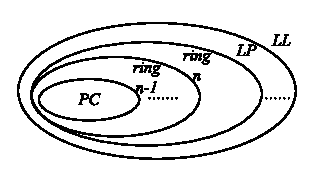
\includegraphics[width=0.3\textwidth]{f123}
\end{center}
\caption{Relationship between $PC$,$LP$ and $LL$}
  \label{f123}
\end{figure}



\section{Preliminaries}\label{sec_prem}

\subsection{Basic Notation of Propositional Satisfiability Problem}\label{subsec_SAT}
\begin{figure}[t]
\begin{center}
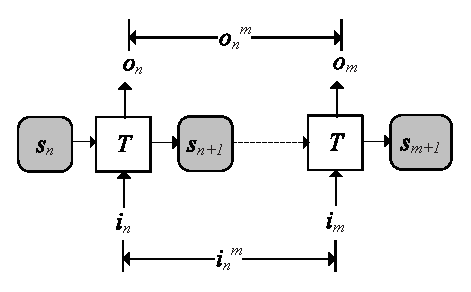
\includegraphics[width=0.35\textwidth]{mealy}
\end{center}
\caption{Mealy finite state machine}
  \label{mealy}
\end{figure}

For a Boolean formula $F$ over a variable set $V$,
the \textbf{Propositional Satisfiability Problem}(abbreviated as \textbf{SAT}) is to find a satisfying assignment $A:V\to \{0,1\}$,
so that $F$ can be evaluated to 1.
If such a satisfying assignment exists, then $F$ is \textbf{satisfiable};
otherwise,
it is \textbf{unsatisfiable}.

A computer program that decides the existence of such a satisfying assignment is called a \textbf{SAT solver},
such as Zchaff\cite{CHAFF}, Grasp\cite{grasp}, Berkmin\cite{BERKMIN},
and MiniSAT\cite{EXTSAT}.
A formula to be solved by a SAT solver is also called a \textbf{SAT instance}.

\subsection{Recurrence Diameter}

A circuit can be modeled by \textbf{Kripke structure} $M=(S,I$ $,T,A,L)$,
with a finite state set $S$,
the initial state set $I\subseteq S$,
the transition relation $T\subseteq S\times S$,
and the labeling of the states $L:S\rightarrow 2^{A}$ with atomic proposition set $A$.

Kroening et al. \cite{RecDiam} defined the \textbf{state variables recurrence diameter} with respect to $M$,
denoted by $rrd(M)$,
as the longest loop-free path in $M$ starting from an initial state.

\begin{equation}\label{equ_svrd}
\begin{split}
&rrd(M)\overset{def}{=}\max\{i|\exists s_0 \dots s_i:\\
& I(s_0)\wedge \bigwedge^{i-1}_{j=0}T(s_j,s_{j+1})\wedge\bigwedge^{i-1}_{j=0}\bigwedge^{i}_{k=j+1}s_{j}\ne s_{k}\}
\end{split}
\end{equation}

In this paper,
we define a similar concept: the \textbf{uninitialized state variables recurrence diameter} with respect to $M$,
denoted by $uirrd(M)$,
is the longest loop-free path in $M$.
%}

\begin{equation}\label{equ_uisvrd}
\begin{split}
&uirrd(M)\overset{def}{=}\max\{i|\exists s_0 \dots s_i:\\
&\bigwedge^{i-1}_{j=0}T(s_j,s_{j+1})\wedge\bigwedge^{i-1}_{j=0}\bigwedge^{i}_{k=j+1}s_{j}\ne s_{k}\}
\end{split}
\end{equation}

The only difference between these two definitions is that
our $uirrd$ does not consider the initial state.

These definitions are only used in proving our theorems below.
Our algorithm does not need to compute these diameters.

\subsection{The Original Algorithm to Determine the Existence of Decoder}\label{subsec_chkextdec}
The complementary synthesis algorithm\cite{ShengYuShen:iccad09} includes two steps:
determining the existence of decoder and characterizing its Boolean function.
We will only introduce the first step here.

The encoder $E$ can be modeled by a Mealy finite state machine \cite{MEALY}.

\begin{definition11}\label{MealyFSM}%\addtolength{\itemsep}{-0.5\baselineskip}
%{\setlength{\baselineskip}{0.5\baselineskip}
\textbf{Mealy finite state machine} is a 5-tuple $M=(S,s_0,I,O,T)$,
consisting of a finite state set $S$,
an initial state $s_0\in S$,
a finite set of input letters $I$,
a finite set of output letters $O$,
a transition function $T: S\times I\to S\times O$ that computes the next state and output letter from the current state and input letter.
%}
\end{definition11}

As shown in Figure \ref{mealy},
as well as in the remainder of this paper,
the state is represented as a gray round corner box,
and the transition function $T$ is represented by a white rectangle.

We denote the state, input letter and output letter at the $n$-th cycle respectively as $s_n$, $i_n$ and $o_n$.
We further denote the sequence of state, input letter and output letter from the $n$-th to the $m$-th cycle respectively as $s_n^m$, $i_n^m$ and $o_n^m$.

A sufficient condition for the existence of $E^{-1}$ is the \textbf{unique condition},
i.e.,
there exist two parameters $d$ and $l$,
so that $i_n$ of $E$ can be uniquely determined by the output sequence $o_{n+d-l}^{n+d-1}$.
As shown in Figure \ref{t1},
$d$ is the relative delay between $o_{n+d-l}^{n+d-1}$ and the input letter $i_n$,
while $l$ is the length of $o_{n+d-l}^{n+d-1}$.

\begin{figure}[b]
\begin{center}
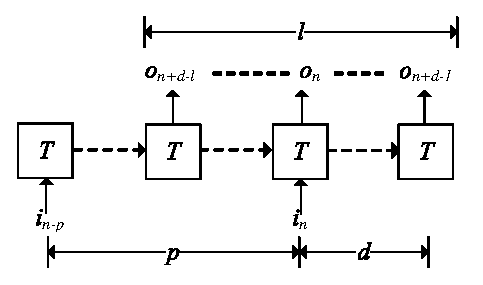
\includegraphics[width=0.4\textwidth]{t1}
\end{center}
\caption{The parameterized complementary condition}
  \label{t1}
\end{figure}

However,
the unique condition is unnecessarily restrictive,
because it may not hold when $s_n$ is not reachable,
even if $E$ is a correct encoder whose input can be uniquely determined by its output in its reachable state set.
So we need to rule out unreachable states before checking the unique condition.

The continuous running character of communication circuits provides us an opportunity to rule out unreachable states easily without paying the expensive cost of computing the reachable state set.
That is to say,
we only need to check the unique condition on the state set $RS^{\infty}$ that can be reached infinitely often from $S$.

\begin{equation}
RS^{q}\overset{def}{=} \{s_q|\bigwedge_{m=0}^{q-1}\{(s_{m+1},o_m)\equiv T(s_m,i_m)\}\}
\end{equation}
\begin{equation}
RS^{>p}\overset{def}{=}\bigcup_{q>p} RS^{q}
\end{equation}
\begin{equation}\label{rse}
RS^{\infty}\overset{def}{=}\lim_{p\rightarrow\infty}RS^{>p}
\end{equation}

Here,
$RS^{q}$ is the set of states that can be reached from $S$ with exact $q$ steps.

According to Equation (\ref{rse}) and Figure \ref{t1},
$RS^{\infty}$ can be easily over-approximated by prepending a state transition sequence of length $p$ to $s_{n}$,
which forces $s_{n}$ to be in the state set $RS^{>p}=\bigcup_{q>p} RS^{q}$.
Obviously,
$RS^{\infty}$ and all $RS^{>p}$ form a total order shown below,
which means a tighter over-approximation of $RS^{\infty}$ can be obtained by increasing the length $p$ of prepended state transition sequence.

\begin{displaymath}
RS^{\infty}\subseteq\dots \subseteq RS^{>p2}\subseteq\dots \subseteq RS^{> p1}\subseteq\dots \textrm{  where } p2>p1
\end{displaymath}

Thus,
as shown in Figure \ref{t1},
the parameterized complementary condition($PC$)\cite{ShengYuShen:iccad09} can be defined as:

\begin{definition11}\label{def_pcc}%\addtolength{\itemsep}{-0.5\baselineskip}
%{\setlength{\baselineskip}{0.5\baselineskip}
\textbf{Parameterized Complementary Condition ($\boldsymbol{PC}$) :}
For encoder $E$,
$E\vDash PC(p,d,l)$ holds if
$i_n$ can be uniquely determined by $o_{n+d-l}^{n+d-1}$ on $s_{n-p}^{n+d-1}$.
This equals the unsatisfiability of $F_{PC}(p,d,l)$ in Equation (\ref{uniqt1}).
We further define $E\vDash PC$ as $\exists p,d,l:E\vDash PC(p,d,l)$.
%When $E$ is clear in the context,
%we just write $PC$ or $PC(p,d,l)$.
%Other notations are:

%1. $E\nvDash PC(p,d,l)\quad \overset{def}{=}\quad \neg \{E\vDash PC(p,d,l)\}$

%2. $E\vDash PC\quad\quad\quad\quad \overset{def}{=}\quad \exists p,d,l:E\vDash PC(p,d,l)$

%3. $E\nvDash PC\quad\quad\quad\quad \overset{def}{=}\quad \neg \{E\vDash PC\}$
%}
\end{definition11}

\begin{equation}\label{uniqt1}
\begin{split}
&F_{PC}(p,d,l)\overset{def}{=}\\
&\left\{
\begin{array}{c}
\bigwedge_{m=n-p}^{n+d-1}
\{
(s_{m+1},o_m)\equiv T(s_m,i_m)
\}
\\
\wedge\quad\bigwedge_{m=n-p}^{n+d-1}
\{
(s'_{m+1},o'_m)\equiv T(s'_m,i'_m)
\}
\\
\wedge\quad\bigwedge_{m=n+d-l}^{n+d-1}o_m\equiv o'_m \\
\wedge\quad i_n\ne i'_n
\end{array}
\right\}
\end{split}
\end{equation}

%This definition is the same as that of Subsection \ref{subsec_chkextdec} and paper \cite{ShengYuShen:iccad09}.

The 2nd and 3rd lines of Equation (\ref{uniqt1}) correspond respectively to two unfolded instances of $E$'s transition function.
The only difference between them is that a prime is appended to every variable in the 3rd line.
The 4th line forces the output sequences of these two unfolded instances to be the same,
while the 5th line forces their input letters to be different.

\section{Case Studies}\label{sec_case}
To facilitate the understanding of our idea,
we use some small examples shown in Figure \ref{fig_case1},\ref{fig_case2} and \ref{fig_case3}.

\subsection{Case study 1}\label{subsec_case1}

\begin{figure}[b]
\begin{center}
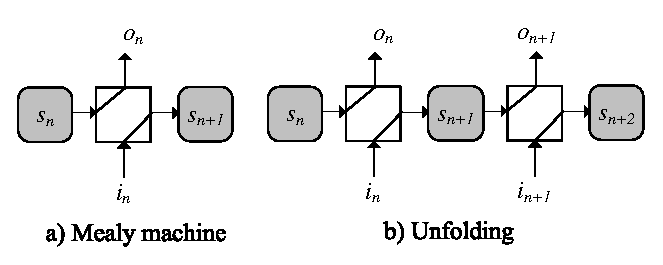
\includegraphics[width=0.45\textwidth]{c1}
\end{center}
\caption{Case study 1}
  \label{fig_case1}
\end{figure}

The circuit in Figure \ref{fig_case1}a) stores its input port $i_n$ in register $s_{n+1}$,
and then outputs it to output port $o_{n+1}$.
The unfolding of its transition function is shown in Figure \ref{fig_case1}b).

Obviously,
$i_n$ is same as,
and therefore can be uniquely determined by $s_{n+1}$.
So $i_n$ can be uniquely determined by $s_n$, $o_n$ and $s_{n+1}$.
So $LP$ is satisfied by this circuit.
Here,
the tuple $<s_n, o_n, s_{n+1}>$ can be seen as a ring that surrounds $i_n$.

Next,
we expand the ring $<s_n, o_n, s_{n+1}>$ to another ring $<s_n, o_n, o_{n+1}, s_{n+2}>$,
and perform the following 3 checks:
\begin{enumerate}
\item Whether $i_n$ can be uniquely determined by the ring $<s_n, o_n, o_{n+1}, s_{n+2}>$?
Obviously the answer is yes.
\item Whether $i_n$ can be uniquely determined by $<o_n, o_{n+1}, s_{n+2}>$, the ring with $s_n$ removed?
Obviously the answer is yes.
\item Whether $i_n$ can be uniquely determined by $<o_n, o_{n+1}>$, the ring with $s_n$ and $s_{n+2}$ both removed?
Obviously the answer is yes.
In this case,
we find that $i_n$ can be uniquely determined by the output sequence $<o_n, o_{n+1}>$.
Thus,
a decoder exists for this circuit.
\end{enumerate}

\subsection{Case study 2}\label{subsec_case2}

\begin{figure}[t]
\begin{center}
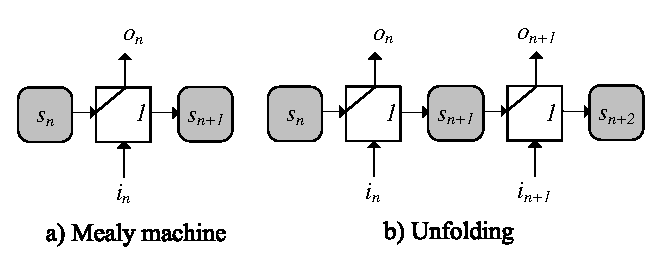
\includegraphics[width=0.45\textwidth]{c2}
\end{center}
\caption{Case study 2}
  \label{fig_case2}
\end{figure}

The circuit in Figure \ref{fig_case2}a) connects a constant 1,
instead of input port $i$ to register $s$.
So $i_n$ can never be determined by $s_n$, $o_n$ and $s_{n+1}$ in all states.
Thus,
a loop-like path with length 1 will reach such a state,
which satisfies $LL$ and falsifies $LP$.
So no decoder exists for this circuit.

\subsection{Case study 3}\label{subsec_case3}

\begin{figure}[b]
\begin{center}
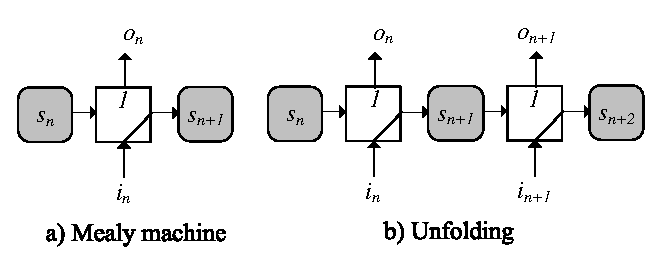
\includegraphics[width=0.45\textwidth]{c3}
\end{center}
\caption{Case study 3}
  \label{fig_case3}
\end{figure}

For the circuit in Figure \ref{fig_case3}a),
the unfolding of its transition function is shown in Figure \ref{fig_case3}b).
It's output is driven by constant 1,
instead of register $s$.
Obviously,
this circuit can satisfy $LP$,
which means $i_n$ can be uniquely determined by $s_n$,$o_n$ and $s_{n+1}$.

Next,
we expand the ring $<s_n, o_n, s_{n+1}>$ to another ring $<s_n, o_n, o_{n+1}, s_{n+2}>$,
and perform the following 3 checks:
\begin{enumerate}
\item Whether $i_n$ can be uniquely determined by the ring $<s_n, o_n, o_{n+1}, s_{n+2}>$?
The answer is no,
because $i_n$ never goto $o_n$, $o_{n+1}$ and $s_{n+2}$.
\item Whether $i_n$ can be uniquely determined by $<o_n, o_{n+1}, s_{n+2}>$, the ring with $s_n$ removed?
The answer is still no with the same reason.
\item Whether $i_n$ can be uniquely determined by $<o_n, o_{n+1}>$, the ring with $s_n$ and $s_{n+2}$ both removed?
The answer is still no with the same reason.
\end{enumerate}
So in this case,
no more expansion is needed,
no decoder exists for this circuit.


\section{Over-approximating $PC$ with $LP$ and Falsifying $LP$ by Searching for Loop-like Path}\label{sec_t2t3}

\subsection{Definition of Over-approximation}\label{subsec_loopdef}

We first present some related definitions before defining the over-approximation of $PC$.

\begin{definition11}\label{def_uniqstate}%\addtolength{\itemsep}{-0.5\baselineskip}
%{\setlength{\baselineskip}{0.5\baselineskip}
\textbf{Unique State Set $\boldsymbol{S^{U}}$ and Non-unique State Set $\boldsymbol{S^{N}}$:}
For a circuit $E$,
its unique state set $\boldsymbol{S^{U}}$ is the set of states $s_{n}$ that makes $i_n$ to be uniquely determined by $s_n$,$o_n$ and $s_{n+1}$,
i.e.,
makes $F^U$ in Equation (\ref{eq_uniqstate}) unsatisfiable.
The non-unique state set $S^{N}$ is the complementary set of $S^{U}$,
i.e.,
$\boldsymbol{S^{N}\overset{def}{=}S-S^{U}}$.
\end{definition11}

\begin{figure}[t]
\begin{center}
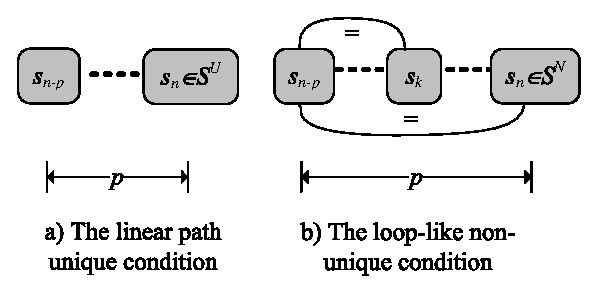
\includegraphics[width=0.4\textwidth]{t2t3}
\end{center}
\caption{Two new uniqueness conditions}
  \label{t2t3}
\end{figure}

\begin{equation}\label{eq_uniqstate}
\begin{split}
&F^U\overset{def}{=}\\
&\left\{
\begin{array}{c}
(s_{n+1},o_n)\equiv T(s_n,i_n)
\\
\wedge(s'_{n+1},o'_n)\equiv T(s'_n,i'_n)
\\
\wedge o_n\equiv o'_n\wedge s_n\equiv s'_n\wedge s_{n+1}\equiv s'_{n+1} \\
\wedge i_n\ne i'_n
\end{array}
\right\}
\end{split}
\end{equation}
%
%The following definitions define three types of unique conditions,
%including $PC$, $LP$ and $LL$,
%in a more formal presentation style with the symbols $\vDash$ and $\nvDash$ borrowed from model checking.

To obtain a halting algorithm,
we need to develop a negative condition for $PC$,
which can recognize all those $E\vDash\neg PC$.

Unfortunately,
it is very difficult,
if not impossible,
to develop such a condition.
So we choose to first over-approximate $PC$ with the linear path unique condition($LP$),
and then develop a negative condition for $LP$,
i.e.,
the loop-like non-unique condition($LL$).
The definitions of $LP$ and $LL$ are given below,
and presented intuitively in Figure \ref{t2t3}a) and \ref{t2t3}b).

\begin{definition11}\label{def_lfuc}%\addtolength{\itemsep}{-0.5\baselineskip}
%{\setlength{\baselineskip}{0.5\baselineskip}
\textbf{Linear Path Unique Condition ($\boldsymbol{LP}$) :}
For encoder $E$,
$E\vDash LP(p)$ holds if
every linear path of length $p$ always reaches the unique state set $S^{U}$.
This equals the unsatisfiability of $F_{LP}(p)$ in Equation (\ref{uniqt2}).
We further define $E\vDash LP$ as $\exists p:E\vDash LP(p)$.
%When $E$ is clear in the context,
%we just write $LP$ or $LP(p)$.
%Other notations are:

%1. $E\nvDash LP(p)\quad \overset{def}{=}\quad \neg \{E\vDash LP(p)\}$

%2. $E\vDash LP\quad\quad \overset{def}{=}\quad \exists p:E\vDash LP(p)$

%3. $E\nvDash LP\quad\quad \overset{def}{=}\quad \neg \{E\vDash LP\}$
%}
\end{definition11}

\begin{equation}\label{uniqt2}
F_{LP}(p)\overset{def}{=} F^U\\
\wedge
\bigwedge_{m=n-p}^{n}
\{
(s_{m+1},o_m)\equiv T(s_m,i_m)
\}
\end{equation}

%\begin{figure}[t]
%\begin{center}
%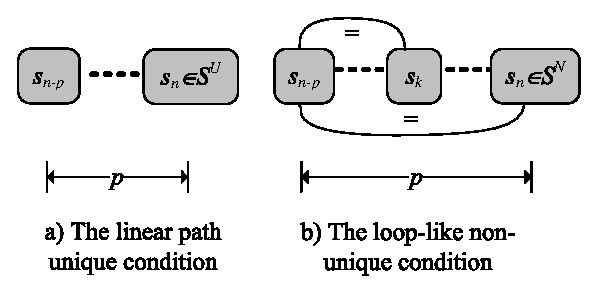
\includegraphics[width=0.5\textwidth]{t2t3}
%\end{center}
%\caption{The linear path unique condition and loop-like non-unique condition}
%  \label{t2}
%\end{figure}

%The 2nd line of Equation (\ref{uniqt2}) is an unfolded instance of $E$,
%from the $(n-p)$-th to the $n$-th cycle.
%The 3rd line is another unfolded instance of $E$,
%with only the $n$-th cycle.
%The 4th line forces the current state, output letter and next state of the two unfolded instances at $n$-th cycle to be the same.
%The last line forces the $i_n$ and $i'_n$ to be different.

\begin{definition11}\label{def_llnc}%\addtolength{\itemsep}{-0.5\baselineskip}
%{\setlength{\baselineskip}{0.5\baselineskip}
\textbf{Loop-like Non-unique Condition ($\boldsymbol{LL}$) :}
For encoder $E$,
$E\vDash LL(p)$ holds if
there exists a loop-like path of length $p$ that reaches the non-unique state set $S^{N}$.
This equals the satisfiability of $F_{LL}(p)$ in Equation (\ref{uniqt3}).
We further define $E\vDash LL$ as $\exists p:E\vDash LL(p)$.
%When $E$ is clear in the context,
%we just write $LL$ or $LL(p)$.
%Other notations are:

%1. $E\nvDash LL(p)\quad \overset{def}{=}\quad \neg \{E\vDash LL(p)\}$

%2. $E\vDash LL\quad\quad \overset{def}{=}\quad \exists p:E\vDash LL(p)$

%3. $E\nvDash LL\quad\quad \overset{def}{=}\quad \neg \{E\vDash LL\}$
%}
\end{definition11}

%\begin{equation}\label{uniqt3}
%\begin{split}
%&F_{LL}(p)\overset{def}{=}\\
%&\left\{
%\begin{array}{c}
%\bigwedge_{m=n-p}^{n}
%\{
%(s_{m+1},o_m)\equiv T(s_m,i_m)
%\}
%\\
%\wedge(s'_{n+1},o'_n)\equiv T(s'_n,i'_n)
%\\
%\wedge o_n\equiv o'_n\wedge s_n\equiv s'_n\wedge s_{n+1}\equiv s'_{n+1} \\
%\wedge i_n\ne i'_n \\
%\wedge\quad \bigvee_{m=n-p+1}^{n}\{s_m\equiv s_{n-p}\}
%\end{array}
%\right\}
%\end{split}
%\end{equation}

\begin{equation}\label{uniqt3}
F_{LL}(p)\overset{def}{=}F_{LP}(p)\wedge\bigvee_{m=n-p+1}^{n}\{s_m\equiv s_{n-p}\}
\end{equation}

Equation (\ref{uniqt3}) is very similar to Equation (\ref{uniqt2}),
except that $\bigvee_{m=n-p+1}^{n}\{s_m\equiv s_{n-p}\}$ is inserted to find a loop-like path.

The intuition behind $LP$ and $LL$ is to check
whether $i_n$ can be uniquely determined by $s_n$,$s_{n+1}$ and $o_n$ with prepended $s_{n-p}^{n-1}$.
Here,
parameters $d$ and $l$ are removed,
which makes it easier to find the value of $p$ .


%\begin{figure}[t]
%\begin{center}
%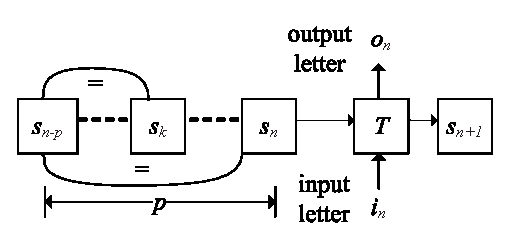
\includegraphics[width=0.4\textwidth]{t3}
%\end{center}
%\caption{The loop-like non-unique condition}
%  \label{t3}
%\end{figure}

%\subsection{Another Formula that Defines $LP$}
%To further discuss the relationship between $PC$ and $LP$,
%we need to define a new formula $\overline{F}_{LP}(p,d,l)$,
%which will be proved equal to $F_{LP}(p)$.


\subsection{Relationships between $PC$, $LP$ and $LL$}\label{subsec_relproof}

The relationships between $PC$, $LP$ and $LL$ are :
%\begin{enumerate}

1. $LP$ over-approximates $PC$,i.e.,$E\vDash PC\to E\vDash LP$.

2. Between $LP$ and $LL$,
there is always one and only one that holds,i.e.,$E\vDash LP\leftrightarrow E\vDash\neg LL$.

%3. At least one of $LP$ and $LL$ holds,i.e.,$E\vDash LP\vee E\vDash LL$.
%\end{enumerate}

These relationships are presented intuitively in Figure \ref{f123},
and their proofs are presented below.
Those impatient readers can skip the remainder of this subsection.

%\begin{lemma}\label{largerl}
%$E\vDash PC(p,d,l)\to E\vDash PC(p,d,l+1)$
%\end{lemma}
%\begin{IEEEproof}
%According to Equation (\ref{uniqt1}),
%it is obvious that:
%
%\begin{displaymath}
%F_{PC}(p,d,l+1)=F_{PC}(p,d,l)\wedge \quad o_{n+d-l-1}\equiv o'_{n+d-l-1}
%\end{displaymath}
%
%So the unsatisfiability of $F_{PC}(p,d,l)$ implies the unsatisfiability of $F_{PC}(p,d,l+1)$.
%Thus we have $E\vDash PC(p,d,l)\to E\vDash PC(p,d,l+1)$
%%\IEEEQED
%\end{IEEEproof}
%\smallskip
%\smallskip
%
%So while discussing $F_{PC}(p,d,l)$ and $E\vDash PC(p,d,l)$,
%we can increase $l$ to any value we like,
%which means we can always assume $l>d$.

Before proving these theorems,
we need a lemma that defines a new formula for $LP$.

\begin{lemma}\label{t2t2new}
With $\overline{F}_{LP}(p,d,l)$ defined below:
\begin{equation}\label{uniqt2_simt1_3}
\begin{split}
&\overline{F}_{LP}(p,d,l)\overset{def}{=}\\
&\left\{
\begin{array}{c}
\bigwedge_{m=n-p}^{n+d-1}
\{
(s_{m+1},o_m)\equiv T(s_m,i_m)
\}
\\
\wedge\quad\bigwedge_{m=n-p}^{n+d-1}
\{
(s'_{m+1},o'_m)\equiv T(s'_m,i'_m)
\}
\\
\wedge o_n\equiv o'_n\wedge s_n\equiv s'_n\wedge s_{n+1}\equiv s'_{n+1} \\
\wedge i_n\ne i'_n
\end{array}
\right\}
\end{split}
\end{equation}
we have:
$\overline{F}_{LP}(p,d,l)\leftrightarrow F_{LP}(p)$
\end{lemma}
\begin{IEEEproof}
\textbf{First,
for the $\to$ direction.}
It is obvious that the clause set of $\overline{F}_{LP}(p,d,l)$ is a supper set of $F_{LP}(p)$,
so the $\to$ direction is proved.

\textbf{Second,
to prove the $\gets$ direction,}
we list below all additional sub-formulas that have been added into Equation (\ref{uniqt2}) to obtain (\ref{uniqt2_simt1_3}),
and also our methods to satisfy them with a particular satisfying assignment $A$ of $F_{LP}(p)$.

1. $\bigwedge_{m=n-p}^{n}\{(s'_{m+1},o'_m)\equiv T(s'_m,i'_m)\}$: This formula can be satisfied by assigning $A(s_m)$, $A(i_m)$ and $A(o_m)$ to $s'_m$, $i'_m$ and $o'_m$ respectively.

2. $\bigwedge_{m=n+1}^{n+d-1}\{(s_{m+1},o_m)\equiv T(s_m,i_m)\}$:
this formula represents a state transition sequence starting from $s_{n+1}$,
which is satisfiable.

3. $\bigwedge_{m=n+1}^{n+d-1}\{(s'_{m+1}$ $,o'_m)\equiv T(s'_m,i'_m)\}$:
this formula represents a state transition sequence starting from $s'_{n+1}$,
which is satisfiable with the same assignment defined in 2.

So,
every satisfying assignment $A$ of $F_{LP}(p)$ can make $\overline{F}_{LP}(p,d,l)$ satisfiable.
So the $\gets$ direction is proved.

Thus, this theorem is proved.
%\IEEEQED
\end{IEEEproof}

In the remainder of this paper,
we will use $F_{LP}(p)$ and $\overline{F}_{LP}(p,d,l)$ interchangeably.

\begin{theorem}\label{R1}
$E\vDash PC(p,d,l)\to E\vDash LP(p)$
\end{theorem}
\begin{IEEEproof}
Let's prove it by contradiction.
Assume that $A:V\to \{0,1\}$ is a satisfying assignment of $\overline{F}_{LP}(p,d,l)$.

%We can append a sub-formula $\bigwedge_{m=n+1}^{n+d-1}
%\{
%(s_{m+1},o_m)\equiv T(s_m,i_m)
%\}$
%to ${F_{LP}(p)}$,
%and obtain:
%
%\begin{equation}\label{uniqt2_simt1_1}
%\begin{split}
%&F'_{LP}(p)\overset{def}{=}\\
%&\left\{
%\begin{array}{c}
%\bigwedge_{m=n-p}^{n+d-1}
%\{
%(s_{m+1},o_m)\equiv T(s_m,i_m)
%\}
%\\
%\wedge(s'_{n+1},o'_n)\equiv T(s'_n,i'_n)
%\\
%\wedge o_n\equiv o'_n\wedge s_n\equiv s'_n\wedge s_{n+1}\equiv s'_{n+1} \\
%\wedge i_n\ne i'_n
%\end{array}
%\right\}
%\end{split}
%\end{equation}
%
%In Equation (\ref{uniqt2_simt1_1}),
%the newly appended sub-formula represents a state transition sequence starting from $s_{n+1}$,
%so $F'_{LP}(p)$ is still satisfiable.
%
%Similarly,
%we can append another sub-formula $\bigwedge_{m=n+1}^{n+d-1}
%\{
%(s'_{m+1},o'_m)\equiv T(s'_m,i'_m)
%\}$ to the 3rd line of Equation (\ref{uniqt2_simt1_1}),
%and obtain a new satisfiable formula:
%
%\begin{equation}\label{uniqt2_simt1_11}
%\begin{split}
%&F''_{LP}(p)\overset{def}{=}\\
%&\left\{
%\begin{array}{c}
%\bigwedge_{m=n-p}^{n+d-1}
%\{
%(s_{m+1},o_m)\equiv T(s_m,i_m)
%\}
%\\
%\bigwedge_{m=n}^{n+d-1}
%\{
%(s'_{m+1},o'_m)\equiv T(s'_m,i'_m)
%\}
%\\
%\wedge o_n\equiv o'_n\wedge s_n\equiv s'_n\wedge s_{n+1}\equiv s'_{n+1} \\
%\wedge i_n\ne i'_n
%\end{array}
%\right\}
%\end{split}
%\end{equation}
%
%We can prepend a third sub-formula $\bigwedge_{m=n-p}^{n-1}
%\{
%(s'_{m+1},o'_m)\equiv T(s'_m,i'_m)
%\}$ to the 3rd line of Equation (\ref{uniqt2_simt1_11}),
%and get a new formula :
%
%\begin{equation}\label{uniqt2_simt1_2}
%\begin{split}
%&F'''_{LP}(p)\overset{def}{=}\\
%&\left\{
%\begin{array}{c}
%\bigwedge_{m=n-p}^{n+d-1}
%\{
%(s_{m+1},o_m)\equiv T(s_m,i_m)
%\}
%\\
%\wedge \bigwedge_{m=n-p}^{n+d-1}
%\{
%(s'_{m+1},o'_m)\equiv T(s'_m,i'_m)
%\}
%\\
%\wedge o_n\equiv o'_n\wedge s_n\equiv s'_n\wedge s_{n+1}\equiv s'_{n+1} \\
%\wedge i_n\ne i'_n
%\end{array}
%\right\}
%\end{split}
%\end{equation}
%
%Because of $s_n\equiv s'_n$ in line 4 of Equation (\ref{uniqt2_simt1_2}),
%this newly prepended sub-formula represents a state transition sequence $s'^{n}_{n-p}$ that reaches $s'_n$,
%which means it can be satisfied by the same satisfying assignment of $s^{n}_{n-p}$.
%So $F'''_{LP}(p)$ is still satisfiable.
%
%Assume that $A'$ is a satisfying assignment of the satisfiable formula $F'_{LP}(p)$ in Equation (\ref{uniqt2_simt1_1}).
We define a new satisfying assignment $A'$ as:
\begin{equation}
A'(v) \overset{def}{=} \left\{ \begin{array}{ll}
A(o_m) & v\equiv o'_m\quad m\neq n \\
A(i_m) & v\equiv i'_m\quad m\neq n \\
A(s_m) & v\equiv s'_m\quad m\neq n\quad and\quad m\neq n+1 \\
A(v) & otherwise
\end{array}
\right.
\end{equation}

Thus,
$A'$ is also a satisfying assignment of $\overline{F}_{LP}(p,d,l)$.

By comparing Equation (\ref{uniqt1}) with (\ref{uniqt2_simt1_3}),
it is obvious that $A'$ is a satisfying assignment of the unsatisfiable formula ${F_{PC}(p,d,l)}$.

This contradiction concludes the proof.
%\IEEEQED
\end{IEEEproof}

\begin{theorem}\label{T2toT3}
$E\vDash LP\leftrightarrow E\vDash\neg LL$
\end{theorem}
\begin{IEEEproof}
\textbf{For the $\to$ direction},
let's prove it by contradiction.
Assume that $E\vDash LL$.
This means there exists a loop-like path that reaches state $s_n\in S^{N}$.

Assume the length of this loop is $q$,
and the parameter of $E\vDash LP$ is $p$.
Then we can unfold this loop $[p/q]+1$ times,
to get a path that is longer than $p$
and reaches a state $s_n\in S^{N}$.
This will lead to $E\vDash\neg LP(p)$.

This contradiction concludes the proof of the $\to$ direction.

\textbf{For the $\gets$ direction},
assume that $E\vDash\neg LP$ and $E\vDash\neg LL$,
then for all $p$,
$F_{LP}(p)$ is satisfiable.

Assume the uninitialized state variables recurrence diameter of $E$ is $uirrd$,
and let $p=uirrd+1$.
Then $F_{LP}(p)$ is satisfiable,
which means there is a path of length $p$ that reaches a state $s_n\in S^{N}$.
Because $p$ is larger than $uirrd$,
this path must contain a loop in it,
which also makes $F_{LL}$ satisfiable.

So $E\vDash LL$ holds,
which contradicts with $E\vDash\neg LL$.

This contradiction concludes the proof of the $\gets$ direction.
%\IEEEQED
\end{IEEEproof}

\subsection{Algorithm to Check $E\vDash LP$ and $E\vDash LL$}\label{subsec_t1t2}
Based on the relationships discussed in Subsection \ref{subsec_relproof},
we develop Algorithm \ref{algo_T2T3}(as shown below) to check $E\vDash LP$ and $E\vDash LL$.
This algorithm also discovers the value of parameter $p$ if $E\vDash LP$ holds.

\begin{algorithm}
\caption{checkLPLL}
\label{algo_T2T3}
\begin{algorithmic}[1]
\FOR{$p=0 \to \infty$}
\IF{$F_{LP}(p)$ is unsatisfiable}
\PRINT \texttt{"$E\vDash LP(p)$"}\label{lab_t2}
\STATE \textbf{halt};
\ELSIF{$F_{LL}(p)$ is satisfiable}
\PRINT \texttt{"no $E^{-1}$ due to $E\vDash LL(p)$"}\label{lab_t3}
\STATE \textbf{halt};
\ENDIF
\ENDFOR
\end{algorithmic}
\end{algorithm}

According to Theorem \ref{T2toT3},
Algorithm \ref{algo_T2T3} will eventually halt at line \ref{lab_t2} or \ref{lab_t3} before $p$ reaches $E$'s uninitialized state variables recurrence diameter $uirrd$.
Thus,
we have the following theorem.

\begin{theorem}\label{a1h}
Algorithm \ref{algo_T2T3} is a halting algorithm.
\end{theorem}

With Algorithm \ref{algo_T2T3},
we can determine whether $E$ is an improperly designed encoder that leads to $E\vDash LL$.
\textbf{But if $E\vDash LP$, how to determine whether $E$ is a correct encoder that leads to $E\vDash PC$}?
We will discuss this problem in the next section.


\section{Checking $E\vDash PC$ by Constructing Onion-Ring}\label{sec_t1t2}
\subsection{Intuitive Description}\label{subsec_intuitive}
\begin{figure}[b]
\begin{center}
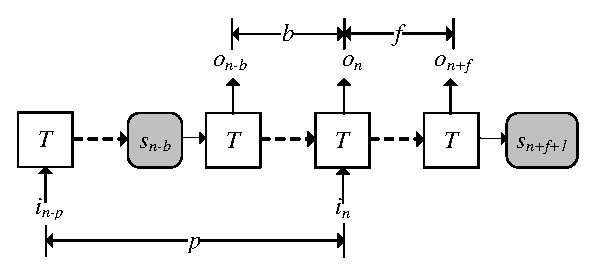
\includegraphics[width=0.5\textwidth]{lr}
\end{center}
\caption{Forward and backward constraints}
  \label{lr}
\end{figure}

To make it easier to follow our presentation,
we present our idea intuitively here with an example.

As shown in Figure \ref{lr},
we add two new parameters $b$ and $f$ to replace $d$ and $l$.
The backward parameter $b$ refers to the distance between state $s_{n-b}$ and $s_n$.
The forward parameter $f$ refers to the distance between state $s_{n+1}$ and $s_{n+1+f}$.
The relations between $<b,f>$ and $<d,l>$ are:

\begin{equation}\label{eq_bfdl}
\begin{split}
&d=f\\
&l=b+f+1
\end{split}
\end{equation}

Because Algorithm \ref{algo_T2T3} already recognizes all $E$s that lead to $E\vDash LL$,
we only need to deal with those $E$s that lead to $E\vDash LP(p)$ here.
This will result in the following proposition:

\begin{proposition}\label{p1}
$i_n$ is uniquely determined by $s_n$, $o_n$ and $s_{n+1}$.
\end{proposition}

As shown in Figure \ref{lr},
we can further generalize Proposition \ref{p1} by:
\begin{enumerate}
\item Replacing $o_n$ with $o_{n-b}^{n+f}$,
\item Replacing $s_n$ with $s_{n-b}$,
\item Replacing $s_{n+1}$ with $s_{n+f+1}$,
\end{enumerate}
and thus obtain:
\begin{proposition}\label{p2}
$i_n$ is uniquely determined by $s_{n-b}$, $o_{n-b}^{n+f}$ and $s_{n+f+1}$.
\end{proposition}

It is obvious that Proposition \ref{p1} is a special case of Proposition \ref{p2},
with $b\equiv 0$ and $f\equiv 0$.

With this generalization,
our algorithm will be intuitively described in the following five steps:


\begin{enumerate}
\item First,
we ignore both $s_{n-b}$ and $s_{n+f+1}$,
and test whether $i_n$ can be uniquely determined by $o_{n-b}^{n+f}$.
\textbf{If yes,
our algorithm halts with $E\vDash PC$}.

\item Otherwise,
we ignore $s_{n-b}$,
and test whether $i_n$ can be uniquely determined by $o_{n-b}^{n+f}$ and $s_{n+f+1}$.
If yes,
then $i_n$ definitely does \textbf{NOT} depend on any $o_k$ with $k<n-b$,
but it may still depend on some $o_k$ with $k>n+f$.
So we need to increase $f$ by 1 and goto step 1.

\item Otherwise,
we ignore $s_{n+f+1}$,
and test whether $i_n$ can be uniquely determined by $s_{n-b}$ and $o_{n-b}^{n+f}$.
If yes,
then $i_n$ definitely does \textbf{NOT} depend on any $o_k$ with $k>n+f$,
but it may still depend on some $o_k$ with $k<n-b$.
So we need to increase $b$ by 1 and goto step 1.

\item Otherwise,
we test whether $i_n$ can be uniquely determined by $s_{n-b}$, $o_{n-b}^{n+f}$ and $s_{n+f+1}$.
If yes,
then $i_n$ may depend on some $o_k$ with both $k<n-b$ and $k>n+f$,
so we need to increase $b$ and $f$ by 1,
and goto step 1.

\item If the algorithm reaches here,
then $i_n$ had been uniquely determined by $s_{n-b'}$, $o_{n-b'}^{n+f'}$ and $s_{n+f'+1}$ previously,
but \textbf{NOT} by $s_{n-b}$, $o_{n-b}^{n+f}$ and $s_{n+f+1}$ now,
where $b'\le b$ and $f'\le f$.
This means that adding more $o_k$ into $o_{n-b}^{n+f}$ by increasing $b$ and $f$, will never make $PC$ holds.
\textbf{Our algorithm halts with $E\vDash\neg PC$}.
\end{enumerate}

In this algorithm,
every step with a pair of $b$ and $f$ corresponds to an onion-ring defined in subsection \ref{subsec_onionring}.
%If the algorithm halts at step 1,
%then $E^{-1}$ exists.
If it halts at step 5,
then $E$ belongs to the ring corresponding to $b'$ and $f'$,
but does not belong to the next inner ring corresponding to $b$ and $f$,
which means $E^{-1}$ does not exist.

Formal presentation and proof will be given in the next two subsections.

\subsection{Constructing Onion-Ring between $PC$ and $LP$}\label{subsec_onionring}

According to Figure \ref{lr},
we define the following formulas:

$F_{unfold}$ defines two unfolded instances of transition function,
and constrains that their output sequence are equivalent,
whereas their input letters are inequivalent:

\begin{equation}\label{F_unfold}
\begin{split}
&F_{unfold}(p,b,f)\overset{def}{=}\\
&\left\{
\begin{array}{c}
\bigwedge_{m=n-p}^{n+f}
\{
(s_{m+1},o_m)\equiv T(s_m,i_m)
\}
\\
\wedge\quad\bigwedge_{m=n-p}^{n+f}
\{
(s'_{m+1},o'_m)\equiv T(s'_m,i'_m)
\}
\\
\bigwedge_{m=n-b}^{n+f}\{o_m\equiv o'_m\}
\\
\wedge\quad i_n\ne i'_n
\end{array}
\right\}
\end{split}
\end{equation}

$F_{backward}$ constrains that $s_{n-b}$ equals $s'_{n-b}$:
\begin{equation}\label{F_b}
F_{backward}(p,b,f) \overset{def}{=}\{s_{n-b}\equiv s'_{n-b}\}
\end{equation}

$F_{forward}$ constrains that $s_{n+1+f}$ equals $s'_{n+1+f}$:
\begin{equation}\label{F_f}
F_{forward}(p,b,f) \overset{def}{=}\{s_{n+1+f}\equiv s'_{n+1+f}\}
\end{equation}

%$F_{output}$ constrains that $<o_{n-b},\dots,o_{n+f}>$ equals $<o'_{n-b},\dots,o'_{n+f}>$:
%\begin{equation}\label{F_o}
%F_{output}(p,b,f) \overset{def}{=}\bigwedge_{m=n-b}^{n+f}\{o_m\equiv o'_m\}
%\end{equation}

With these formulas,
we define 4 new unique conditions between $PC$ and $LP$.

%\textbf{$\boldsymbol{LP\_nobf(p,b,f)}$: linear path unique condition without backward and forward constraints}:
%Every state $s_n$ reached by a linear path of length $p$
% can always make $i_n$ to be uniquely determined by $<o_{n-b},\dots,o_{n+f}>$,
%i.e.,
%make $F_{LP\_nobf}$ in Equation (\ref{t2_nobf}) unsatisfiable.

\textbf{$\boldsymbol{LP\_nobf(p,b,f)}$}:
$i_n$ can be uniquely determined by $o_{n-b}^{n+f}$.
This equals the unsatisfiability of $F_{LP\_nobf}$ in Equation (\ref{t2_nobf}).

\begin{equation}\label{t2_nobf}
F_{LP\_nobf}(p,b,f)\overset{def}{=} F_{unfold}
\end{equation}

\textbf{$\boldsymbol{LP\_f(p,b,f)}$}:
$i_n$ can be uniquely determined by $o_{n-b}^{n+f}$ and $s_{n+1+f}$.
This equals the unsatisfiability $F_{LP\_f}$ in Equation (\ref{t2_f}).
%\textbf{$\boldsymbol{LP\_f(p,b,f)}$: linear path unique condition with forward constraint only}:
%Every state $s_n$ reached by a linear path of length $p$
% can always make $i_n$ to be uniquely determined by $<o_{n-b},\dots,o_{n+f}>$ and $s_{n+1+f}$,
%i.e.,
%make $F_{LP\_f}$ in Equation (\ref{t2_f}) unsatisfiable.

\begin{equation}\label{t2_f}
F_{LP\_f}(p,b,f)\overset{def}{=} F_{unfold}\wedge F_{forward}
\end{equation}

\textbf{$\boldsymbol{LP\_b(p,b,f)}$}:
$i_n$ can be uniquely determined by $s_{n-b}$ and $o_{n-b}^{n+f}$.
This equals the unsatisfiability $F_{LP\_b}$ in Equation (\ref{t2_b}).

%\textbf{$\boldsymbol{LP\_b(p,b,f)}$: linear path unique condition with backward constraint only}:
%Every state $s_n$ reached by a linear path of length $p$
% can always make $i_n$ to be uniquely determined by $s_{n-b}$ and $<o_{n-b},\dots,o_{n+f}>$,
%i.e.,
%make $F_{LP\_b}$ in Equation (\ref{t2_b}) unsatisfiable.

\begin{equation}\label{t2_b}
F_{LP\_b}(p,b,f)\overset{def}{=} F_{unfold}\wedge F_{backward}
\end{equation}

%\textbf{$\boldsymbol{LP\_bf(p,b,f)}$: linear path unique condition with backward and forward constraints}:
%Every state $s_n$ reached by a linear path of length $p$
% can always make $i_n$ to be uniquely determined by $s_{n-b}$, $<o_{n-b},\dots,o_{n+f}>$ and $s_{n+1+f}$,
%i.e.,
%make $F_{LP\_bf}$ in Equation (\ref{t2_bf}) unsatisfiable.

\textbf{$\boldsymbol{LP\_bf(p,b,f)}$}:
$i_n$ can be uniquely determined by $s_{n-b}$, $o_{n-b}^{n+f}$ and $s_{n+1+f}$.
This equals the unsatisfiability $F_{LP\_bf}$ in Equation (\ref{t2_bf}).

\begin{equation}\label{t2_bf}
F_{LP\_bf}(p,b,f)\overset{def}{=} F_{unfold}\wedge F_{backward}\wedge F_{forward}
\end{equation}

These new unique conditions,
when coupled with parameters $b$ and $f$,
will act as onion-rings between $PC$ and its over-approximation $LP$.

It is obvious that,
$LP\_bf$ is very similar to $LP$,
while $LP\_nobf$ is very similar to $PC$.
Such similarities will be employed to prove the correctness of our approach.

Some lemmas that will bed used to prove the correctness of the onion-ring approach are given below:

\begin{lemma}\label{lma_bfinc}
$E\vDash LP\_bf(p,b,f)\gets E\vDash LP\_bf(p,b,f+1)$
\end{lemma}
\begin{IEEEproof}
Let's prove it by contradiction.
Assume that $E\vDash\neg LP\_bf(p,b,f)$ and $E\vDash LP\_bf(p,b,f+1)$,
which means that $F_{LP\_bf}(p,b,f)$ is satisfiable while $F_{LP\_bf}(p,b,f+1)$ is unsatisfiable.

We can append a state transition to $F_{LP\_bf}(p,b,f)$ after $s_{n+f+1}$,
and get a new formula $F'_{LP\_bf}(p,b,f)$.
\begin{equation}
\begin{split}
&F'_{LP\_bf}(p,b,f)\overset{def}{=}F_{LP\_bf}(p,b,f)\\
&\wedge(s_{n+f+2},o_{n+f+1})=T(s_{n+f+1},i_{n+f+1})
\end{split}
\end{equation}

This newly appended state transition is satisfiable,
which makes $F'_{LP\_bf}$ a satisfiable formula.

Assume $A$ is a satisfying assignment of $F'_{LP\_bf}(p,b,f)$.
We define another satisfying assignment $A'$ as

\begin{equation}
A'(v) \overset{def}{=} \left\{ \begin{array}{ll}
A(o_{n+f+1}) & v\equiv o'_{n+f+1} \\
A(i_{n+f+1}) & v\equiv i'_{n+f+1} \\
A(s_{n+f+2}) & v\equiv s'_{n+f+2} \\
A(v) & otherwise
\end{array}
\right.
\end{equation}

Obviously,
$A'$ is a satisfying assignment of unsatisfiable formula $F_{LP\_bf}(p,b,f+1)$.

This contradiction concludes the proof.
%\IEEEQED
\end{IEEEproof}

\begin{lemma}\label{lma_binc}
$E\vDash LP\_b(p,b,f)\gets E\vDash LP\_b(p+1,b+1,f)$
\end{lemma}

Its proof is similar to that of Lemma \ref{lma_bfinc}.

\begin{lemma}\label{lma_gets1}
If $E\vDash PC(p,d,l)$,
then the following Equation holds.
\begin{equation}\label{eq_gets1}
\begin{array}{llll}
&E\vDash& LP\_bf&(p+d-l+1,0,d) \\
\leftrightarrow&E\vDash& LP\_b&(p+d-l+1,0,d) \\
\end{array}
\end{equation}
\end{lemma}
\begin{IEEEproof}
%Actually we need to prove :
%\begin{equation}\label{eq_gets1_1}
%F_{LP\_bf}(p+d-l,0,d)\leftrightarrow F_{LP\_b}(p+d-l,0,d)
%\end{equation}
\textbf{For the $\gets$ direction},
according to Equation (\ref{t2_b}) and (\ref{t2_bf}),
it is obvious that the clause set of $F_{LP\_bf}$ is a super set of $F_{LP\_b}$,
which means the unsatisfiability of the latter one implies the unsatisfiability of the former one.
So the $\gets$ direction is proved.

\textbf{For the $\to$ direction},
let's prove it by contradiction.
Assume that $F_{LP\_bf}(p+d-l+1,0,d)$ is unsatisfiable,
and $A$ is a satisfying assignment of $F_{LP\_b}(p+d-l+1,0,d)$.

We define another assignment $A'$ as :
\begin{equation}
A'(v) \overset{def}{=} \left\{ \begin{array}{ll}
A(o_{k}) & v\equiv o'_{k}\quad where\quad k<n \\
A(i_{k}) & v\equiv i'_{k}\quad where\quad k<n \\
A(s_{k}) & v\equiv s'_{k}\quad where\quad k<n \\
A(v) & otherwise
\end{array}
\right.
\end{equation}

Obviously,
$A'$ is a satisfying assignment of Equation (\ref{uniqt1}),
which means $E\nvDash PC(p,d,l)$.
This contradiction concludes the proof of the $\to$ direction.

%\IEEEQED
\end{IEEEproof}

\begin{lemma}\label{lma_gets2}
If $E\vDash PC(p,d,l)$,
then the following Equation holds.
\begin{equation}\label{eq_gets2}
\begin{array}{llll}
&E\vDash& LP\_b&(p,l-d-1,d) \\
\leftrightarrow&E\vDash& LP\_nobf&(p,l-d-1,d) \\
\end{array}
\end{equation}
\end{lemma}

Its proof is similar to that of Lemma \ref{lma_gets1}.

An important theorem that defines the onion-ring is presented and proved below:

\begin{theorem}\label{thm_onionring}
If $E\vDash PC(p,d,l)$,
then there exists a list of unique conditions with their relationship shown below:
\begin{equation}\label{eq_onionring}
\begin{array}{llll}
&E\vDash& LP&(p+d-l+1)\\
\leftrightarrow&E\vDash& LP\_bf&(p+d-l+1,0,0) \\
\gets&E\vDash& LP\_bf&(p+d-l+1,0,1) \\
&& \dots &\\
\gets&E\vDash& LP\_bf&(p+d-l+1,0,d-1) \\
\gets&E\vDash& LP\_bf&(p+d-l+1,0,d) \\
\leftrightarrow&E\vDash& LP\_b&(p+d-l+1,0,d) \\
\gets&E\vDash& LP\_b&(p+d-l+2,1,d) \\
&& \dots &\\
\gets&E\vDash& LP\_b&(p,l-d-1,d) \\
%\gets&E\vDash& LP\_b&(p,l-d,d) \\
\leftrightarrow&E\vDash& LP\_nobf&(p,l-d-1,d) \\
\leftrightarrow&E\vDash&PC&(p,d,l)
\end{array}
\end{equation}
\end{theorem}
\begin{IEEEproof}
According to Equation (\ref{uniqt2_simt1_3}) and (\ref{t2_bf}),
the $\boldsymbol{\leftrightarrow}$ relation between the 1st and 2nd line of Equation (\ref{eq_onionring}) holds.

According to Lemma \ref{lma_bfinc},
the $\boldsymbol{\gets}$ relations between the 2nd and 6th line of Equation (\ref{eq_onionring}) holds.

According to Lemma \ref{lma_gets1},
the $\boldsymbol{\leftrightarrow}$ relation between the 6th and 7th line of Equation (\ref{eq_onionring}) holds.

According to Lemma \ref{lma_binc},
the $\boldsymbol{\gets}$ relations between the 7th and 10th line of Equation (\ref{eq_onionring}) holds.

According to Lemma \ref{lma_gets2},
the $\boldsymbol{\leftrightarrow}$ relation between the 10th and 11th line of Equation (\ref{eq_onionring}) holds.

According to Equation (\ref{uniqt1}) and (\ref{t2_nobf}),
the $\boldsymbol{\leftrightarrow}$ relations between the last two lines of Equation (\ref{eq_onionring}) holds.
%\IEEEQED
\end{IEEEproof}

In Equation (\ref{eq_onionring}),
all $\gets$ symbols form a total order,
which makes all unique conditions on the right-hand side of $\vDash$s to form an onion-ring(as shown in Figure \ref{f123}).

\subsection{Algorithm Implementation}

With those theorems presented in Subsection \ref{subsec_onionring},
we use the following Algorithm \ref{algo_T1T2} to check $E\vDash PC$.

\begin{algorithm}
\caption{$checkPCLP(p,b,f)$}
\label{algo_T1T2}
\begin{algorithmic}[1]
\IF{$F_{LP\_nobf}(p,b,f)$ is unsatisfiable}
\PRINT \texttt{"$E\vDash PC(p,f,b+f+1)$"}\label{lab_t1t2_t2nobf}
\STATE \textbf{halt};
\ELSIF{$F_{LP\_f}(p,b,f)$ is unsatisfiable}
\STATE $checkPCLP(p,b,f+1)$\label{lab_t1t2_t2f}
\ELSIF{$F_{LP\_b}(p,b,f)$ is unsatisfiable}
\STATE $checkPCLP(p+1,b+1,f)$\label{lab_t1t2_t2b}
\ELSIF{$F_{LP\_bf}(p,b,f)$ is unsatisfiable}
\STATE $checkPCLP(p+1,b+1,f+1)$\label{lab_t1t2_t2bf}
\ELSE
\PRINT \texttt{"no $E^{-1}$ due to $E\vDash\neg PC$"}\label{lab_t1t2_sat}
\STATE \textbf{halt};
\ENDIF
\end{algorithmic}
\end{algorithm}

Algorithm \ref{algo_T1T2} is invoked with the form $checkPCLP(p,0,0)$,
with $p$ computed by Algorithm \ref{algo_T2T3}.

Algorithm \ref{algo_T1T2} just follows the onion-ring defined by Equation (\ref{eq_onionring}),
from the first line to the last line.
If $E\vDash PC$ holds,
it will eventually reach line \ref{lab_t1t2_t2nobf},
and the existence of $E^{-1}$ is proved;
otherwise,
it will eventually reach line \ref{lab_t1t2_sat},
which means that $E$ does not belong to the current ring,
and $PC$ is falsified.
So $E^{-1}$ does not exist.

Thus,
with Theorem \ref{thm_onionring},
we have the following theorem.

\begin{theorem}\label{a2h}
Algorithm \ref{algo_T1T2} is a halting algorithm.
\end{theorem}

\section{Removing Redundant Output Letters}\label{sec_rmred}
Although Algorithm \ref{algo_T2T3} and \ref{algo_T1T2} together are sufficient to determine the existence of $E^{-1}$,
the parameters found by line \ref{lab_t1t2_t2nobf} of Algorithm \ref{algo_T1T2} contain some redundancy,
which will cause unnecessary large overhead of circuit area.

\begin{figure}[b]
\begin{center}
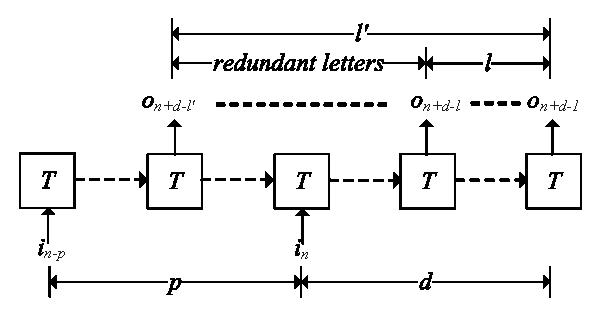
\includegraphics[width=0.45\textwidth]{rmred}
\end{center}
\caption{Redundant Output Letters}
  \label{fig_rmred}
\end{figure}

For example,
as shown in Figure \ref{fig_rmred},
assume that $l$ is the smallest parameter value that leads to $E\vDash PC(p,d,l)$,
and $l<d$,
which means that $i_n$ is uniquely determined by some output letters $o_k$ with $k>n$.

We further assume that line \ref{lab_t1t2_t2nobf} of Algorithm \ref{algo_T1T2} find out $E\vDash PC(p,d,l')$.
It is obvious that $l'>d$,
which make $i_n$ to depend on some redundant $o_k$ with $k\le n$.

So $o_{n+d-l'}^{n+d-l-1}$ is the sequence of redundant output letters,
which should be removed to prevent them from being instantiated as latches in circuit $E^{-1}$.

Algorithm \ref{algo_remove} that removes these redundant output letters is presented below:

\begin{algorithm}
\caption{$RemoveRedundancy(p,d,l')$}
\label{algo_remove}
\begin{algorithmic}[1]
\FOR{$l=0 \to l'$}
\IF{$F_{PC}(p,d,l)$ is unsatisfiable}
\PRINT \texttt{"$E\vDash PC(p,d,l)$"}
\STATE \textbf{halt};
%\ELSE
%\STATE \textbf{continue};
\ENDIF
\ENDFOR
\end{algorithmic}
\end{algorithm}

\section{Experimental Results}\label{sec_exp}
We have implemented our algorithm in Zchaff\cite{CHAFF},
and run it on a PC with a 2.4GHz Intel Core 2 Q6600 processor, 8GB memory and CentOS 5.2 linux.
All experimental results and programs can be downloaded from \url{http://www.ssypub.org}.
%All related programs and data files can be downloaded from \url{http://www.ssypub.org}.
\subsection{Benchmarks}
\begin{table}[t]
\centering
\caption{Information of Benchmarks}
\begin{tabular}{|c|c|c|c|c|c|}
\hline
&XGXS&XFI&scrambler&PCIE&T2 et-\\
&&&&&hernet\\\hline
Line number&&&&&\\
of verilog&214&466&24&1139&1073\\
source code&&&&&\\\hline
\#regs&15&135&58&22&48\\\hline
Data path&8&64&66&10&10\\
width&&&&&\\ \hline
\end{tabular}
\end{table}


Table \Rmnum{1} shows information of the following benchmarks.
\begin{enumerate}

\item A XGXS encoder compliant to clause 48 of IEEE-802.3ae 2002 standard \cite{IEEE80232002}.

\item A XFI encoder compliant to clause 49 of the same IEEE standard.

\item A 66-bit scrambler used to ensure
that a data sequence has sufficiently many 0-1 transitions
, so that it can run through high-speed
noisy serial transmission channel.

\item A PCIE physical coding module.

\item The Ethernet module of Sun's OpenSparc T2 processor.
\end{enumerate}

\subsection{Experimental Results on Properly Designed Encoders}
\begin{table}[b]
\centering
\caption{Experimental Results on Properly Designed Encoders}
\begin{tabular}{|c|c|c|c|c|c|c|}
\hline
&                                        &XGXS     &XFI       &scra-     &PCIE    &T2 et-\\
&                                        &         &          &mbler     &        &hernet\\ \hline
&time chk                           &&&&&\\
&$PC$(sec)                               &0.49     &59.19     &2.52      &1.46    &35.17\\\cline{2-7}
&$d,p,l$                                 &1,0,1    &0,3,2     &0,1,2     &2,1,1   &4,0,1         \\ \cline{2-7}
\cite{ShengYuShen:iccad09}&run time      &         &          &          &        &              \\
&allsat(sec)                             &1.16     &1047.19   &2.00      &0.96    &29.51       \\\cline{2-7}
&area                                    &765      &19443     &1455      &398     &648           \\ \hline\hline
&time chk                         &&&&&\\
&$PC$(sec)                               &1.32     &88.68     &7.23      &2.73    &84.47\\\cline{2-7}
&$d,p,l$                                 &1,1,1    &0,3,2     &0,2,2     &2,1,1   &4,1,1          \\ \cline{2-7}
Ours&run time                            &         &          &          &        &              \\
&allsat(sec)                             &1.38     &1055.64   &3.23      &1.18    &29.42              \\\cline{2-7}
&area                                    &773      &19481     &1455      &400     &535          \\ \hline
\end{tabular}
\end{table}

The 2nd and 6th rows of Table \Rmnum{2} compares the run time of checking $E\vDash PC$ between \cite{ShengYuShen:iccad09} and our approach.
The run time of our approach are much larger than \cite{ShengYuShen:iccad09}.
This is caused by checking the unique and non-unique conditions defined in Section \ref{sec_t2t3} and \ref{sec_t1t2}.

The 3rd and 7th rows compare the discovered parameter values,
and some minor differences are found on parameter $p$.
This is caused by the different orders in checking various parameter combinations.

According to \cite{ShengYuShen:tcad},
$p$ is used to constrain the reachable states,
while $d$ and $l$ will affect the run time of building $E^{-1}$ and its circuit area.
To prove this,
we compared the run time of building $E^{-1}$ with all-solution SAT solver in the 4th and 8th rows of Table \Rmnum{2},
and also compared the area of $E^{-1}$ in the 5th and 9th rows.
These $E^{-1}$s were synthesized with DesignCompiler and LSI10 target library.


The results indicate that the differences in parameter $p$ do not cause significant overhead in the run time of all-solution SAT solver and circuit area.

\begin{table}[t]
\centering
\caption{Experimental Results on Improperly Designed Encoders}
\begin{tabular}{|c|c|c|c|c|c|}
\hline
&XGXS&XFI&scra-&PCIE&T2 et-\\
&&&mbler&&hernet\\ \hline
Alg 1 result   &$LP(1)$    &$LL(2)$     &$LL(2)$     &$LP(1)$   &$LP(1)$         \\\hline
Alg 2 result   &$\neg PC$       &NA     &NA        &$\neg PC$   &$\neg PC$          \\ \hline
time(sec)           &1.23      &44.58     &3.26      &1.67     &21.49          \\ \hline
\end{tabular}
\end{table}
\subsection{Experimental Results on Improperly Designed Encoders}
To further show the usefulness of our algorithm,
we need some improperly designed encoders without corresponding decoders.

We obtained these improperly designed encoders by modifying each benchmark's output statements,
such that they can explicitly output the same letter for two different input letters.
In this way,
input letter $i_n$ can never be uniquely determined by $E$'s output sequence.

The 2nd row of Table \Rmnum{3} shows the result of Algorithm \ref{algo_T2T3},
while the 3rd row shows the result of Algorithm \ref{algo_T1T2}.
The total run time is shown in the 4th row.

For XFI and scrambler,
the result of Algorithm 1 is $LL$,
which falsifies $PC$ directly.
So the result of Algorithm 2 is \textbf{NA}.

The results indicate that our algorithm always terminated,
and recognized these modified incorrect encoders.

%Following are the results of checking these modified encoders:
%\begin{enumerate}

%1. XGXS:
%algorithm \ref{algo_T2T3} found out $E\vDash LP(1)$,
%but algorithm \ref{algo_T1T2} found out $E\nvDash PC$.
%The run time was 1.23 seconds.
%
%2. XFI:
%algorithm \ref{algo_T2T3} found out $E\vDash LL$.
%The run time was 44.58 seconds.
%
%3. Scrambler:
%algorithm \ref{algo_T2T3} found out $E\vDash LL$.
%The run time was 3.26 seconds.
%
%4. PCIE:
%algorithm \ref{algo_T2T3} found out $E\vDash LP(1)$,
%but algorithm \ref{algo_T1T2} found out $E\nvDash PC$.
%The run time was 1.67 seconds.
%
%5. T2:
%algorithm \ref{algo_T2T3} found out $E\vDash LP(1)$,
%but algorithm \ref{algo_T1T2} found out $E\nvDash PC$.
%The run time was 21.49 seconds.
%\end{enumerate}


\section{Related Works}\label{sec_relwork}
\subsection{Complementary Synthesis}
%Complementary synthesis is an emerging new research topic,
%there are only two papers that discuss this problem.

The concept of complementary synthesis was first proposed by us\cite{ShengYuShen:iccad09} in ICCAD 2009.
Its major shortcomings are that it is incomplete,
and its run-time overhead of building complementary circuit is too large.

The incomplete problem has been addressed by this paper, while we\cite{ShengYuShen:tcad} addresses the second shortcoming by simplifying the SAT instance with unsatisfiable core extraction before building complementary circuits.

\subsection{The Completeness of Bounded Model Checking}
Bounded model checking(BMC) is a model checking technology that considers only those paths of limited length.
Many researchers try to find out complete approaches for BMC.

One line of research\cite{bmc_tacas99,RecDiam} tries to find out a bound $b$,
which can guarantee the correctness of a specification on all paths,
if the specification is correct on all paths shorter than $b$.

The other line of research\cite{kind_tacas99} tries to find out a pattern for induction,
such that the correctness of a specification within any bound $b$ implies the correctness on bound $b+1$.

Our approach achieves completeness without following these two approaches.
Instead,
we define two complement uniqueness conditions,
$LP$ and $LL$,
and find out proper algorithms to check them.


\subsection{Temporal Logic Synthesis}
%Automatically synthesis of program from logic specification is first identified as Church's problem in 1962\cite{LOGARTHAUTO}.
%Some early researches \cite{SLVSQFSS,AUTOINF} solve this problem by reducing it to checking emptiness of tree automata.

The temporal logic synthesis was first addressed by Clarke et.al\cite{DSGSYNTMPLG} and Manna et.al \cite{SYNTMPLGSPC}.
But Pnueli et.al \cite{SYNRCTVMD} pointed out that the complexity of LTL synthesis is double exponent.
%This high complexity drives researchers turning their focus to find smaller but still useful subset of temporal logic,
%such that synthesis problem can be solved with lower complexity.

One line of research \cite{CNTLSYNTMDAUTO,DTMGENGMELTL,SYNRCTVDES} focuses on the so-called generalized reactive formulas of the form:
$(\square \lozenge p_1 \wedge \cdots \square \lozenge p_m) \to (\square \lozenge q_1 \wedge \cdots \square \lozenge q_n)$.
Complexity of solving synthesis problem for such formula is $O(N^3)$.

The other line of research focuses on finding efficient algorithm \cite{SYNCNTLBNDRPN}
for expensive safra determination algorithm \cite{CMPLXAUTO} on an useful formula subset,
or just avoiding it\cite{NEWALGSTRGSYN}.

%Yet another approach is antichain\cite{ANTICHAIN},
%which reduces the expensive state set computation to computation on maximal and minimal elements of lattice.

Based on these research works,
some tools\cite{ANZU} that can handle small temporal formulas have been developed.

All these works assume a hostile environment,
which seems too restrictive for many applications.
So Fisman et.al \cite{rationalsyn_tacas10}, Chatterjee et.al \cite{assguasyn_tacas07} and Ummels et.al \cite{ralgame_istta06} proposed rational synthesis algorithm,
which assumes that each agents act to achieve their own goals instead of failing each other.


\subsection{Protocol Converter Synthesis}
The protocol converter synthesis was first proposed by Avnit et.al \cite{converter_date08} to automatically generate a translator between two different communication protocols.
Avnit et.al\cite{converter_date09} improved it with a more efficient design space exploration algorithm.
The implementation of this tool is introduced in \cite{converter_tacas10}.

%This paper address the first shortcoming.

\section{Conclusions and Future Works}\label{sec_conclude}

This paper proposes the first halting algorithm that checks whether a particular encoder $E$ has corresponding decoder.
Theoretical analysis and experimental results show that our approach always distinguishes correct encoders from their incorrect variants and halts properly.

One future work is to develop a debugging method to find out why $E^{-1}$ does not exist.
For the failure caused by loop-like path,
we plan to develop a debugging mechanism based on our previous work on loop-like counterexample minimization \cite{ShengYuShen:charme05}.



% An example of a floating figure using the graphicx package.
% Note that \label must occur AFTER (or within) \caption.
% For figures, \caption should occur after the \includegraphics.
% Note that IEEEtran v1.7 and later has special internal code that
% is designed to preserve the operation of \label within \caption
% even when the captionsoff option is in effect. However, because
% of issues like this, it may be the safest practice to put all your
% \label just after \caption rather than within \caption{}.
%
% Reminder: the "draftcls" or "draftclsnofoot", not "draft", class
% option should be used if it is desired that the figures are to be
% displayed while in draft mode.
%
%\begin{figure}[!t]
%\centering
%\includegraphics[width=2.5in]{myfigure}
% where an .eps filename suffix will be assumed under latex,
% and a .pdf suffix will be assumed for pdflatex; or what has been declared
% via \DeclareGraphicsExtensions.
%\caption{Simulation Results}
%\label{fig_sim}
%\end{figure}

% Note that IEEE typically puts floats only at the top, even when this
% results in a large percentage of a column being occupied by floats.


% An example of a double column floating figure using two subfigures.
% (The subfig.sty package must be loaded for this to work.)
% The subfigure \label commands are set within each subfloat command, the
% \label for the overall figure must come after \caption.
% \hfil must be used as a separator to get equal spacing.
% The subfigure.sty package works much the same way, except \subfigure is
% used instead of \subfloat.
%
%\begin{figure*}[!t]
%\centerline{\subfloat[Case I]\includegraphics[width=2.5in]{subfigcase1}%
%\label{fig_first_case}}
%\hfil
%\subfloat[Case II]{\includegraphics[width=2.5in]{subfigcase2}%
%\label{fig_second_case}}}
%\caption{Simulation results}
%\label{fig_sim}
%\end{figure*}
%
% Note that often IEEE papers with subfigures do not employ subfigure
% captions (using the optional argument to \subfloat), but instead will
% reference/describe all of them (a), (b), etc., within the main caption.


% An example of a floating table. Note that, for IEEE style tables, the
% \caption command should come BEFORE the table. Table text will default to
% \footnotesize as IEEE normally uses this smaller font for tables.
% The \label must come after \caption as always.
%
%\begin{table}[!t]
%% increase table row spacing, adjust to taste
%\renewcommand{\arraystretch}{1.3}
% if using array.sty, it might be a good idea to tweak the value of
% \extrarowheight as needed to properly center the text within the cells
%\caption{An Example of a Table}
%\label{table_example}
%\centering
%% Some packages, such as MDW tools, offer better commands for making tables
%% than the plain LaTeX2e tabular which is used here.
%\begin{tabular}{|c||c|}
%\hline
%One & Two\\
%\hline
%Three & Four\\
%\hline
%\end{tabular}
%\end{table}


% Note that IEEE does not put floats in the very first column - or typically
% anywhere on the first page for that matter. Also, in-text middle ("here")
% positioning is not used. Most IEEE journals use top floats exclusively.
% Note that, LaTeX2e, unlike IEEE journals, places footnotes above bottom
% floats. This can be corrected via the \fnbelowfloat command of the
% stfloats package.



%\section{Conclusion}
%The conclusion goes here.





% if have a single appendix:
%\appendix[Proof of the Zonklar Equations]
% or
%\appendix  % for no appendix heading
% do not use \section anymore after \appendix, only \section*
% is possibly needed

% use appendices with more than one appendix
% then use \section to start each appendix
% you must declare a \section before using any
% \subsection or using \label (\appendices by itself
% starts a section numbered zero.)
%


%\appendices
%\section{Proof of the First Zonklar Equation}
%Appendix one text goes here.

% you can choose not to have a title for an appendix
% if you want by leaving the argument blank
%\section{}
%Appendix two text goes here.


% use section* for acknowledgement
\section*{Acknowledgment}
The authors would like to thank the editors and anonymous reviewers for their hard work.

This work was fund by project 60603088 supported by National Natural Science Foundation of China.

This work was also supported by the Program for Changjiang
Scholars and Innovative Research Team in University No
IRT0614.

%The authors would like to thank the anonymous reviewer's time and effort.

%This work is fund by Chinese National Science Foundation No.60603088.


% Can use something like this to put references on a page
% by themselves when using endfloat and the captionsoff option.
\ifCLASSOPTIONcaptionsoff
  \newpage
\fi



% trigger a \newpage just before the given reference
% number - used to balance the columns on the last page
% adjust value as needed - may need to be readjusted if
% the document is modified later
%\IEEEtriggeratref{8}
% The "triggered" command can be changed if desired:
%\IEEEtriggercmd{\enlargethispage{-5in}}

% references section

% can use a bibliography generated by BibTeX as a .bbl file
% BibTeX documentation can be easily obtained at:
% http://www.ctan.org/tex-archive/biblio/bibtex/contrib/doc/
% The IEEEtran BibTeX style support page is at:
% http://www.michaelshell.org/tex/ieeetran/bibtex/
%\bibliographystyle{IEEEtran}
% argument is your BibTeX string definitions and bibliography database(s)
%\bibliography{IEEEabrv,../bib/paper}
%
% <OR> manually copy in the resultant .bbl file
% set second argument of \begin to the number of references
% (used to reserve space for the reference number labels box)
\begin{thebibliography}{1}

\bibitem{ShengYuShen:iccad09}
ShengYu Shen, JianMin Zhang, Ying Qin, SiKun Li.
Synthesizing Complementary Circuits Automatically.
in ICCAD'09,
pp 381-388,
2009.

\bibitem{CHAFF}
M. Moskewicz, C. Madigan, Y. Zhao, L. Zhang, S. Malik.
Chaff: Engineering an Efficient SAT Solver.
In DAC'01,
pp 530-535,
2001.

\bibitem{grasp}
Jo\~ao P. Marques Silva, Karem A. Sakallah.
GRASP - a new search algorithm for satisfiability.
in ICCAD'96,
pp 220-227,
1996.

\bibitem{BERKMIN}
E. Goldberg, Y Novikov.
BerkMin: A Fast and Robust Sat-Solver.
\newpage
in DATE'02,
pp 142-149,
2002.

\bibitem{EXTSAT}
N. E\'en, N. S\"orensson.
Extensible SAT-solver.
in SAT'03,
pp 502-518,
2003.

\bibitem{RecDiam}
D. Kroening, Ofer Strichman.
Efficient Computation of Recurrence Diameters.
in VMCAI'03,
pp 298-309,
2003.

\bibitem{MEALY}
Mealy, George H.
A Method for Synthesizing Sequential Circuits.
Bell Systems Technical Journal v 34, pp 1045-1079, 1955.

\bibitem{IEEE80232002}
\emph{IEEE Standard for Information technology Telecommunications and
  information exchange between systems Local and metropolitan area networks
  Specific requirements Part 3: Carrier Sense Multiple Access with Collision
  Detection (CSMA/CD) Access Method and Physical Layer Specifications
  Amendment: Media Access Control (MAC) Parameters, Physical Layers, and
  Management Parameters for 10 Gb/s Operation}, IEEE Std. 802.3, 2002.

\bibitem{ShengYuShen:tcad}
ShengYu Shen, Ying Qin, KeFei Wang, LiQuan Xiao, JianMin Zhang, SiKun Li.
Synthesizing Complementary Circuits Automatically.
IEEE transaction on CAD of Integrated Circuits and Systems,
29(8):1191-1202,
2010.

\bibitem{bmc_tacas99}
Armin Biere, Alessandro Cimatti, Edmund M. Clarke, Yunshan Zhu.
Symbolic Model Checking without BDDs.
In TACAS'99,
pp 193-207,
1999.

\bibitem{kind_tacas99}
Mary Sheeran, Satnam Singh, Gunnar Stalmarck.
Checking Safety Properties Using Induction and a SAT-Solver.
In FMCAD'00,
pp 108-125,
2000.


\bibitem{DSGSYNTMPLG}
E.M. Clarke, E.A. Emerson.
Design and synthesis of synchronization skeletons using branching time temporal logic.
In IBM Workshop on Logics of Programs,LNCS 131,
pp 52-71,
1981.

\bibitem{SYNTMPLGSPC}
Z. Manna, P. Wolper.
Synthesis of communicating processes from temporal logic specifications.
ACM Trans. Prog. Lang. Sys., 6:68-93, 1984.

\bibitem{SYNRCTVMD}
A. Pnueli, R. Rosner.
On the synthesis of a reactive module.
In Proc. 16th ACM Symp. Princ. of Prog. Lang.,pages 179-190, 1989.

\bibitem{CNTLSYNTMDAUTO}
E. Asarin, O. Maler, A. Pnueli, J. Sifakis.
Controller synthesis for timed automata.
In IFAC Symposium on System Structure and Control, pages 469-474. Elsevier, 1998.

\bibitem{DTMGENGMELTL}
R. Alur, S. La Torre.
Deterministic generators and games for LTL fragments.
ACM Trans. Comput. Log., 5(1):1-25,2004.

\bibitem{SYNRCTVDES}
N. Piterman, A. Pnueli, Y. Saar,
Synthesis of Reactive(1) Designs,
in VMCAI'06,
pp 364-380,
2006.

\bibitem{SYNCNTLBNDRPN}
O. Maler, D. Nickovic, A. Pnueli.
On Synthesizing Controllers from Bounded-Response Properties.
In CAV'07,
pp 95-107,
2007.

\bibitem{CMPLXAUTO}
S. Safra.
Complexity of Automata on Infinite Objects.
PhD thesis, The Weizmann Institute of Science, Rehovot, Israel, March 1989.

\bibitem{NEWALGSTRGSYN}
A. Harding, M. Ryan, P. Schobbens.
A New Algorithm for Strategy Synthesis in LTL Games.
in TACAS'05,
pp 477-492,
2005.

\bibitem{ANZU}
B. Jobstmann, S. Galler, M. Weiglhofer, R. Bloem.
Anzu: A Tool for Property Synthesis.
in CAV'07,
pp 258-262,
2007.

%\bibitem{OPTLTLSYN}
%B. Jobstmann and R. Bloem.
%Optimizations for LTL Synthesis.
%in FMCAD'06,
%pp 117-124,
%2006.

%\bibitem{ANTICHAIN}
%W. Kuijper, J. Pol.
%Computing Weakest Strategies for Safety Games of Imperfect Information.
%In TACAS'09,
%pp 92-106,
%2009.

\bibitem{rationalsyn_tacas10}
D Fisman, O Kupferman, Yoad Lustig.
Rational Synthesis.
in TACAS'10,
pp 190-204,
2010.

\bibitem{assguasyn_tacas07}
Chatterjee, K., Henzinger, T.A. Assume-guarantee synthesis.
In TACAS'07,
pp 261-275,
2007.

\bibitem{ralgame_istta06}
Ummels, M.
Rational behaviour and strategy construction in infinite multiplayer games.
In FSTTCS'06,
pp 212-223,
2006.

\bibitem{converter_date08}
K. Avnit, V. D'Silva, A. Sowmya, S. Ramesh, S. Parameswaran.
A Formal Approach To The Protocol Converter Problem.
in DATE'08,
pp 294-299,
2008.


%\bibitem{converter_todeas09}
%K. Avnit, V. D'Silva, A. Sowmya, S. Ramesh, S. Parameswaran.
%Provably correct on-chip communication: A formal approach to automatic protocol converter synthesis.
%ACM Trans. Design Autom. Electr. Syst. 14(2),
%pp 1-41,
%2009.

\bibitem{converter_date09}
K. Avnit, A. Sowmya.
A formal approach to design space exploration of protocol converters.
in DATE'09,
pp 129-134,
2009.

\bibitem{converter_tacas10}
K. Avnit, A. Sowmya, J. Peddersen.
ACS: Automatic Converter Synthesis for SoC Bus Protocols.
in TACAS'10,
pp 343-348,
2010.

\bibitem{ShengYuShen:charme05}
ShengYu Shen, Ying Qin, Sikun Li.
Minimizing Counterexample of ACTL Property.
in CHARME'05,
pp 393-397,
2005.

\end{thebibliography}

% biography section
%
% If you have an EPS/PDF photo (graphicx package needed) extra braces are
% needed around the contents of the optional argument to biography to prevent
% the LaTeX parser from getting confused when it sees the complicated
% \includegraphics command within an optional argument. (You could create
% your own custom macro containing the \includegraphics command to make things
% simpler here.)
%\begin{biography}[{\includegraphics[width=1in,height=1.25in,clip,keepaspectratio]{mshell}}]{Michael Shell}
% or if you just want to reserve a space for a photo:

%\begin{IEEEbiography}{Michael Shell}
%Biography text here.
%\end{IEEEbiography}

% if you will not have a photo at all:
%\begin{IEEEbiographynophoto}{John Doe}
%Biography text here.
%\end{IEEEbiographynophoto}

% insert where needed to balance the two columns on the last page with
% biographies
%\newpage

%\begin{IEEEbiographynophoto}{Jane Doe}
%Biography text here.
%\end{IEEEbiographynophoto}

% You can push biographies down or up by placing
% a \vfill before or after them. The appropriate
% use of \vfill depends on what kind of text is
% on the last page and whether or not the columns
% are being equalized.

%\vfill

% Can be used to pull up biographies so that the bottom of the last one
% is flush with the other column.
%\enlargethispage{-5in}



% that's all folks
\end{document}


